\chapter{Resultados}
\label{chap:resultados}

\section{Resultados da tabela subject-info.csv}

Inicialmente fiz teste com resultados de dados clínicos de pacientes da tabela subject-info.csv \cite{physionet2020music_dataset} para o processo de análise de dados, e usar como gabarito para depois adaptar os sinais ECG, apliquei um modelo de risco proporcional de cox uma técnica de análise bastante utilizada na área da saúde, meus estudos começou pela regressão de cox mas a comprender melhor os dados percebi que para o meu caso o melhor modelo é o LogisticHazard pelo simples fatos que o regressão de cox trabalho com o tempo continuos e o meu trabalho vai trabalhar com tempo discreto, e o modelo de regressão de cox tem a suposição de proporcionalidade dos riscos que não se aplica ao meu caso, já o modelo LogisticHazard é uma extensão do modelo de regressão de cox para o caso de tempo discreto, porem não vou discartar os resultados que obtive com a regressão de cox, pois os resultados me ajudaram a compreender melhor os dados e o processo de análise, e também me ajudaram a compreender melhor o modelo LogisticHazard, e os resultados obtidos com a regressão de cox foram bastante satisfatórios, e me deram uma boa base para continuar meus estudos com o modelo LogisticHazard,a biblioteca  CoxPHFitter em python  \cite{kvamme2019time} \cite{lifelines_docs_cox} que utiliza métodos de Breslow, que corrigi eventos que ocorreram no mesmo intervalo de tempo. David Cox assumiu que o tempo era contínuo, ou seja, era impossível duas pessoas morrerem no exato mesmo milissegundo. Porem é muito comum dois ou mais pacientes terem o evento no mesmo dia. neste caso o método de Breslow é utilizado para corrigir esses eventos que ocorreram no mesmo intervalo de tempo, o estimador de Breslow ele permite que a Regressão de Cox calcule os pesos $\beta$ mesmo quando a vários eventos no mesmo dia.

Calculo matemático que o modelo CoxPHFitter \cite{lifelines_docs_cox} definem a função de risco do modelo de regressão de cox da seguinte forma:

\begin{equation}
	\label{eq:cox_hazard_eng}
	\underbrace{h(t|x)}_{\text{hazard}} = \overbrace{b_0(t)}^{\text{baseline hazard}} \underbrace{\exp \overbrace{\left( \sum_{i=1}^n b_i(x_i - \overline{x}_i) \right)}^{\text{log-partial hazard}}}_{\text{partial hazard}}
\end{equation}

Onde $b_0(t)$ é a função de risco basal, $b_i$ são os coeficientes de regressão, $x_i$ são as covariáveis e $\overline{x}_i$ são as médias das covariáveis. O modelo de regressão de cox é um modelo sem parâmetros, ou seja, não assume nenhuma forma específica para a função de risco basal, e o modelo de regressão de cox é um modelo semi-paramétrico, pois assume que a função de risco basal é uma função arbitrária, e o modelo de regressão de cox é um modelo multiplicativo, pois assume que a função de risco é multiplicada pela função de risco basal. Quando é semiparametrico o metodo utilizado é Breslow, pois resolve o problema de cox. O modelo de regressão de cox é um modelo de risco proporcional, pois assume que a razão de riscos entre dois indivíduos é constante ao longo do tempo, ou seja, a razão de riscos entre dois indivíduos é dada por:

\begin{equation}
	\label{eq:cox_proportional_hazard_eng}
	\frac{h(t|x_1)}{h(t|x_2)} = \exp \left( \sum_{i=1}^n b_i(x_{1i} - x_{2i}) \right)
\end{equation}


Classifiquei alguns dados em grupo relevante para covariáveis, dados como holter, eletrocardiogramas holter, eventos condicoes cardiovasculares, dados demograficos clinicos, e outros dados de apoio como idade, gênero, esses vão estar presentes em todos dados porque são relevantes para a análise. Analise se baseie em modelo de risco de cox me retornando taxa de risco, intervalo de confiança, matriz de variâncias, erros padrão, log da verossimilhança, com base nos resultados selecionei algumas coveriaveis relevantes para para o treinar junto com os sinais ECG, e tambem comparar o quanto o modelo melhorou com os dados sinais ECG.


Foram avaliadas variáveis derivadas do Holter em modelos de regressão de Cox. As variáveis \textit{Holter available} e \textit{Holter onset (hh:mm:ss)} foram desconsideradas, pois não agregavam informa\c{c}\~ao anal\'itica relevante nesta amostra. A variável \textit{Longest RR pause (ms)} também foi excluída devido à elevada proporção de valores ausentes.



\subsection{Resultados do modelo de Cox para dados Holter}

% -------------------------------------------------------
%  Bloco 1 — Antes das tabelas do Holter
% -------------------------------------------------------

As variáveis do Holter utilizadas na análise estão descritas na
Tabela~\ref{tab:cox_holter_completo}. As variáveis \textit{Holter available}
e \textit{Holter onset} foram desconsideradas por não agregarem informação
analítica relevante — todos os pacientes apresentaram valor igual a 1 na
primeira, e a segunda corresponde apenas ao horário de início do exame.
A variável \textit{Longest RR pause (ms)} também foi excluída em razão da
elevada proporção de valores ausentes (aproximadamente 80\% da amostra).
As demais variáveis consideradas foram: ritmo do Holter
(\textit{Holter rhythm}), intervalos RR mínimo, médio, máximo e amplitude
(\textit{minimum}, \textit{average}, \textit{maximum} e \textit{RR range}),
extrassístoles em dupla (\textit{Extrasystole couplets}), extrassístole
ventricular (\textit{Ventricular Extrasystole}), bradicardia
(\textit{Bradycardia}) e os índices de variabilidade da frequência cardíaca SDNN, SDANN, RMSSD e pNN50. Apresentam-se abaixo dois modelos: o primeiro com a coorte completa ($n=992$) e o segundo com a amostra filtrada para pacientes com as três derivações completas ($n=898$).

Texto texto texto texto texto texto texto texto texto texto texto texto texto texto texto texto texto texto texto texto texto texto texto texto texto texto texto texto texto texto texto texto texto texto texto texto texto texto texto texto texto texto texto texto texto texto texto texto texto texto texto texto texto texto texto texto texto texto texto texto texto texto texto texto texto texto texto texto texto.Texto texto texto texto texto texto texto texto texto texto texto texto texto texto texto texto texto texto texto texto texto texto texto texto texto texto texto texto texto texto texto texto texto texto texto texto texto texto texto texto texto.

Texto texto texto texto texto texto texto texto texto texto texto texto texto texto texto texto texto texto texto texto texto texto texto texto texto texto texto texto texto texto texto texto texto texto texto texto texto texto texto texto texto texto texto texto texto texto texto texto.Texto texto texto texto texto texto texto texto texto texto texto texto texto texto texto texto texto texto texto texto texto.

\begin{table}[htbp]
	\centering
	\caption{Modelo de Cox com variáveis do Holter na coorte completa ($n=992$; 205 eventos).}
	\label{tab:cox_holter_completo}
	\resizebox{\textwidth}{!}{%
		\begin{tabular}{lcccccc}
			\toprule
			Vari\'avel                                & Coef.                                                    & HR   & IC 95\% HR & EP   & $p$      & Signific\^ancia \\
			\midrule
			G\^enero                                  & 0.28                                                     & 1.33 & 0.95--1.85 & 0.17 & 0.10     & N\~ao           \\
			Idade                                     & 0.33                                                     & 1.39 & 1.18--1.64 & 0.08 & $<0.005$ & Sim             \\
			Ritmo Holter\textsuperscript{a}           & 0.15                                                     & 1.17 & 1.02--1.33 & 0.07 & 0.02     & Sim             \\
			RR m\'in. (ms)                            & 0.11                                                     & 1.12 & 0.90--1.39 & 0.11 & 0.32     & N\~ao           \\
			RR m\'ed. (ms)                            & -0.00                                                    & 1.00 & 0.78--1.27 & 0.12 & 0.97     & N\~ao           \\
			RR m\'ax. (ms)                            & -0.01                                                    & 0.99 & 0.70--1.39 & 0.17 & 0.95     & N\~ao           \\
			Amplitude RR (ms)                         & 0.15                                                     & 1.16 & 0.82--1.66 & 0.18 & 0.40     & N\~ao           \\
			Extrasys. em dupla\textsuperscript{b}     & 0.10                                                     & 1.11 & 1.02--1.20 & 0.04 & 0.01     & Sim             \\
			Extrasss\'istole vent.\textsuperscript{c} & 0.23                                                     & 1.26 & 1.07--1.49 & 0.08 & 0.01     & Sim             \\
			Bradicardia                               & -0.03                                                    & 0.97 & 0.83--1.13 & 0.08 & 0.66     & N\~ao           \\
			SDNN (ms)                                 & -0.92                                                    & 0.40 & 0.17--0.93 & 0.44 & 0.03     & Sim             \\
			SDANN (ms)                                & 0.51                                                     & 1.66 & 0.74--3.75 & 0.41 & 0.22     & N\~ao           \\
			RMSSD (ms)                                & 0.31                                                     & 1.37 & 0.96--1.94 & 0.18 & 0.08     & N\~ao           \\
			pNN50 (\%)                                & -0.18                                                    & 0.84 & 0.58--1.20 & 0.18 & 0.33     & N\~ao           \\
			\midrule
			Concordance                               & \multicolumn{6}{c}{0.67}                                                                                         \\
			Partial AIC                               & \multicolumn{6}{c}{2714.94}                                                                                      \\
			Log-likelihood ratio test                 & \multicolumn{6}{c}{72.76 em 14 g.l.; $-\log_2(p)=30.62$}                                                         \\
			\bottomrule
		\end{tabular}%
	}
	\begin{flushleft}
		\footnotesize
		\textsuperscript{a} Ritmo Holter: ritmo cardíaco registrado no Holter (\textit{Holter rhythm}).\\
		\textsuperscript{b} Extrasys. em dupla: extrassístoles em dupla (\textit{Extrasystole couplets}).\\
		\textsuperscript{c} Extrassístole vent.: extrassístole ventricular (\textit{Ventricular Extrasystole}).
	\end{flushleft}
\end{table}

\begin{table}[htbp]
	\centering
	\caption{Modelo de Cox com variáveis do Holter na amostra filtrada com tr\^es deriva\c{c}\~oes completas ($n=898$; 189 eventos).}
	\label{tab:cox_holter_filtrado}
	\resizebox{\textwidth}{!}{%
		\begin{tabular}{lcccccc}
			\toprule
			Vari\'avel                                & Coef.                                                    & HR   & IC 95\% HR & EP   & $p$      & Signific\^ancia \\
			\midrule
			G\^enero                                  & 0.34                                                     & 1.41 & 0.99--2.00 & 0.18 & 0.06     & N\~ao           \\
			Idade                                     & 0.37                                                     & 1.44 & 1.21--1.72 & 0.09 & $<0.005$ & Sim             \\
			Ritmo Holter\textsuperscript{a}           & 0.17                                                     & 1.18 & 1.03--1.36 & 0.07 & 0.02     & Sim             \\
			RR m\'in. (ms)                            & 0.16                                                     & 1.18 & 0.86--1.60 & 0.16 & 0.31     & N\~ao           \\
			RR m\'ed. (ms)                            & -0.03                                                    & 0.97 & 0.75--1.25 & 0.13 & 0.82     & N\~ao           \\
			RR m\'ax. (ms)                            & -0.05                                                    & 0.95 & 0.48--1.88 & 0.35 & 0.89     & N\~ao           \\
			Amplitude RR (ms)                         & 0.21                                                     & 1.24 & 0.58--2.64 & 0.39 & 0.58     & N\~ao           \\
			Extrasys. em dupla\textsuperscript{b}     & 0.10                                                     & 1.11 & 1.02--1.21 & 0.04 & 0.02     & Sim             \\
			Extrasss\'istole vent.\textsuperscript{c} & 0.20                                                     & 1.23 & 1.04--1.45 & 0.09 & 0.02     & Sim             \\
			Bradicardia                               & -0.03                                                    & 0.97 & 0.84--1.14 & 0.08 & 0.75     & N\~ao           \\
			SDNN (ms)                                 & -0.99                                                    & 0.37 & 0.15--0.92 & 0.46 & 0.03     & Sim             \\
			SDANN (ms)                                & 0.55                                                     & 1.73 & 0.74--4.08 & 0.44 & 0.21     & N\~ao           \\
			RMSSD (ms)                                & 0.27                                                     & 1.31 & 0.90--1.91 & 0.19 & 0.16     & N\~ao           \\
			pNN50 (\%)                                & -0.12                                                    & 0.88 & 0.60--1.29 & 0.19 & 0.53     & N\~ao           \\
			\midrule
			Concordance                               & \multicolumn{6}{c}{0.68}                                                                                         \\
			Partial AIC                               & \multicolumn{6}{c}{2461.23}                                                                                      \\
			Log-likelihood ratio test                 & \multicolumn{6}{c}{72.27 em 14 g.l.; $-\log_2(p)=30.32$}                                                         \\
			\bottomrule
		\end{tabular}%
	}
	\begin{flushleft}
		\footnotesize
		\textsuperscript{a} Ritmo Holter: ritmo cardíaco registrado no Holter (\textit{Holter rhythm}).\\
		\textsuperscript{b} Extrasys. em dupla: extrassístoles em dupla (\textit{Extrasystole couplets}).\\
		\textsuperscript{c} Extrassístole vent.: extrassístole ventricular (\textit{Ventricular Extrasystole}).
	\end{flushleft}
\end{table}

\FloatBarrier
\subsubsection{Resumo dos resultados do modelo de Cox para dados Holter}

De modo geral, as duas análises apresentaram resultados consistentes. As variáveis idade, Holter rhythm, Extrasystole couplets, Ventricular Extrasystole e SDNN mantiveram associação estatisticamente significativa com o desfecho nas duas análises. A semelhança entre os achados da coorte completa e da amostra filtrada sugere robustez dos resultados mesmo após a restrição aos pacientes com três derivações completas. O que isso significa é que mesmo com a restrição dos pacientes com três derivações completas, poderei usar essas restriçoes aos sinais de ECG, ao um modelo convulocional resnet, essa filtagem é porque alguns dos pacientes não tem as 3 derivações completas, então a filtragem não atrapallha nos resultados.

\FloatBarrier

% -------------------------------------------------------
%  Bloco 2 — Antes das tabelas de eventos e condições cardiovasculares
% -------------------------------------------------------


\subsection{Resultados do modelo de Cox para dados de eventos e condições cardiovasculares}

As variáveis de eventos e condições cardiovasculares selecionadas para os
modelos reduzidos foram: número de extrassístoles
ventriculares por hora, taquicardia ventricular não sustentada com mais de
dez batimentos (\textit{Non-sustained ventricular tachycardia}, CH$>$10),
número de extrassístoles supraventriculares em 24 horas e taquiarritmia
supraventricular paroxística (\textit{Paroxysmal supraventricular
	tachyarrhythmia}). As variáveis gênero e idade foram incluídas em todos os
modelos como covariáveis de controle padrão.

Para dados de eventos e condições cardiovasculares apresentaram resultados consistentes. Em ambas as análises, apenas idade e taquicardia
ventricular não sustentada (CH$>$10) mantiveram associação estatisticamente
significativa com o desfecho. A semelhança entre os achados da coorte completa
e da amostra filtrada sugere robustez dos resultados mesmo após a restrição
aos pacientes com três derivações completas. Apresentam-se abaixo dois modelos:
o primeiro com a coorte completa ($n=992$) e o segundo com a amostra filtrada
para pacientes com as três derivações completas ($n=898$).

\begin{table}[htbp]
	\centering
	\caption{Modelo de Cox com variáveis arrítmicas na coorte completa ($n=992$; 205 eventos).}
	\label{tab:cox_arritmia_completo}
	\resizebox{\textwidth}{!}{%
		\begin{tabular}{lcccccc}
			\toprule
			Vari\'avel                        & Coef.                                                   & HR   & IC 95\% HR & EP   & $p$      & Signific\^ancia \\
			\midrule
			G\^enero                          & 0.24                                                    & 1.27 & 0.92--1.77 & 0.17 & 0.15     & N\~ao           \\
			Idade                             & 0.35                                                    & 1.42 & 1.21--1.67 & 0.08 & $<0.005$ & Sim             \\
			VE/h\textsuperscript{a}           & 0.02                                                    & 1.02 & 0.90--1.16 & 0.06 & 0.77     & N\~ao           \\
			TVNS (CH$>$10)\textsuperscript{b} & 0.60                                                    & 1.83 & 1.32--2.53 & 0.17 & $<0.005$ & Sim             \\
			SVE/24h\textsuperscript{c}        & -0.01                                                   & 0.99 & 0.88--1.13 & 0.06 & 0.93     & N\~ao           \\
			TASVP\textsuperscript{d}          & 0.11                                                    & 1.12 & 0.98--1.28 & 0.07 & 0.11     & N\~ao           \\
			\midrule
			Concordance                       & \multicolumn{6}{c}{0.64}                                                                                        \\
			Partial AIC                       & \multicolumn{6}{c}{2718.25}                                                                                     \\
			Log-likelihood ratio test         & \multicolumn{6}{c}{53.45 em 6 g.l.; $-\log_2(p)=29.97$}                                                         \\
			\bottomrule
		\end{tabular}%
	}
	\begin{flushleft}
		\footnotesize
		\textsuperscript{a} VE/h: número de extrassístoles ventriculares por hora.\\
		\textsuperscript{b} TVNS: taquicardia ventricular não sustentada (CH$>$10 batimentos).\\
		\textsuperscript{c} SVE/24h: número de extrassístoles supraventriculares em 24 horas.\\
		\textsuperscript{d} TASVP: taquiarritmia supraventricular paroxística.
	\end{flushleft}
\end{table}

\FloatBarrier

\begin{table}[htbp]
	\centering
	\caption{Modelo de Cox com variáveis arrítmicas na amostra filtrada com três derivações completas ($n=898$; 189 eventos).}
	\label{tab:cox_arritmia_filtrado}
	\resizebox{\textwidth}{!}{%
		\begin{tabular}{lcccccc}
			\toprule
			Vari\'avel                        & Coef.                                                   & HR   & IC 95\% HR & EP   & $p$      & Signific\^ancia \\
			\midrule
			G\^enero                          & 0.30                                                    & 1.36 & 0.96--1.92 & 0.18 & 0.09     & N\~ao           \\
			Idade                             & 0.39                                                    & 1.48 & 1.25--1.76 & 0.09 & $<0.005$ & Sim             \\
			VE/h\textsuperscript{a}           & 0.02                                                    & 1.02 & 0.90--1.16 & 0.07 & 0.76     & N\~ao           \\
			TVNS (CH$>$10)\textsuperscript{b} & 0.56                                                    & 1.75 & 1.25--2.44 & 0.17 & $<0.005$ & Sim             \\
			SVE/24h\textsuperscript{c}        & -0.02                                                   & 0.98 & 0.86--1.12 & 0.07 & 0.82     & N\~ao           \\
			TASVP\textsuperscript{d}          & 0.11                                                    & 1.12 & 0.97--1.28 & 0.07 & 0.12     & N\~ao           \\
			\midrule
			Concordance                       & \multicolumn{6}{c}{0.65}                                                                                        \\
			Partial AIC                       & \multicolumn{6}{c}{2464.70}                                                                                     \\
			Log-likelihood ratio test         & \multicolumn{6}{c}{52.80 em 6 g.l.; $-\log_2(p)=29.53$}                                                         \\
			\bottomrule
		\end{tabular}%
	}
	\begin{flushleft}
		\footnotesize
		\textsuperscript{a} VE/h: número de extrassístoles ventriculares por hora.\\
		\textsuperscript{b} TVNS: taquicardia ventricular não sustentada (CH$>$10 batimentos).\\
		\textsuperscript{c} SVE/24h: número de extrassístoles supraventriculares em 24 horas.\\
		\textsuperscript{d} TASVP: taquiarritmia supraventricular paroxística.
	\end{flushleft}
\end{table}

\FloatBarrier

\subsection{Resultados do modelo de Cox para dados demográficos clínicos}

As variáveis demográficas e clínicas avaliadas foram: peso corporal
(\textit{Weight}, kg), altura (\textit{Height}, cm), índice de massa corporal
(IMC, kg/m\textsuperscript{2}) e classe funcional da New York Heart Association
(NYHA). As variáveis idade e gênero, embora pertençam a este grupo, foram
excluídas desta listagem específica por já estarem presentes como covariáveis
de controle em todos os modelos analisados.


\begin{table}[htbp]
	\centering
	\caption{Modelo de Cox com dados clínicos e antropométricos na coorte completa ($n=992$; 205 eventos).}
	\label{tab:cox_clinico_completo}
	\resizebox{\textwidth}{!}{%
		\begin{tabular}{lcccccc}
			\toprule
			Vari\'avel                & Coef.                                                   & HR   & IC 95\% HR & EP   & $p$      & Signific\^ancia \\
			\midrule
			G\^enero                  & 0.65                                                    & 1.92 & 1.28--2.88 & 0.21 & $<0.005$ & Sim             \\
			Idade                     & 0.29                                                    & 1.34 & 1.14--1.57 & 0.08 & $<0.005$ & Sim             \\
			Peso (kg)                 & 0.03                                                    & 1.03 & 0.25--4.26 & 0.72 & 0.97     & N\~ao           \\
			Altura (cm)               & -0.23                                                   & 0.79 & 0.34--1.83 & 0.43 & 0.59     & N\~ao           \\
			IMC\textsuperscript{a}    & -0.26                                                   & 0.77 & 0.23--2.58 & 0.62 & 0.67     & N\~ao           \\
			Classe NYHA               & 0.93                                                    & 2.54 & 1.90--3.39 & 0.15 & $<0.005$ & Sim             \\
			\midrule
			Concordance               & \multicolumn{6}{c}{0.67}                                                                                        \\
			Partial AIC               & \multicolumn{6}{c}{2693.46}                                                                                     \\
			Log-likelihood ratio test & \multicolumn{6}{c}{78.24 em 6 g.l.; $-\log_2(p)=46.79$}                                                         \\
			\bottomrule
		\end{tabular}%
	}
	\begin{flushleft}
		\footnotesize
		\textsuperscript{a} IMC: índice de massa corporal (kg/m\textsuperscript{2}).
	\end{flushleft}
\end{table}

\begin{table}[htbp]
	\centering
	\caption{Modelo de Cox com dados clínicos e antropométricos na amostra filtrada com três derivações completas ($n=898$; 189 eventos).}
	\label{tab:cox_clinico_filtrado}
	\resizebox{\textwidth}{!}{%
		\begin{tabular}{lcccccc}
			\toprule
			Vari\'avel                & Coef.                                                   & HR   & IC 95\% HR & EP   & $p$      & Signific\^ancia \\
			\midrule
			G\^enero                  & 0.74                                                    & 2.09 & 1.37--3.20 & 0.22 & $<0.005$ & Sim             \\
			Idade                     & 0.33                                                    & 1.38 & 1.17--1.64 & 0.09 & $<0.005$ & Sim             \\
			Peso (kg)                 & 0.15                                                    & 1.16 & 0.27--5.05 & 0.75 & 0.85     & N\~ao           \\
			Altura (cm)               & -0.32                                                   & 0.73 & 0.31--1.73 & 0.44 & 0.47     & N\~ao           \\
			IMC\textsuperscript{a}    & -0.36                                                   & 0.70 & 0.20--2.45 & 0.64 & 0.58     & N\~ao           \\
			Classe NYHA               & 0.93                                                    & 2.53 & 1.87--3.41 & 0.15 & $<0.005$ & Sim             \\
			\midrule
			Concordance               & \multicolumn{6}{c}{0.68}                                                                                        \\
			Partial AIC               & \multicolumn{6}{c}{2438.61}                                                                                     \\
			Log-likelihood ratio test & \multicolumn{6}{c}{78.89 em 6 g.l.; $-\log_2(p)=47.23$}                                                         \\
			\bottomrule
		\end{tabular}%
	}
	\begin{flushleft}
		\footnotesize
		\textsuperscript{a} IMC: índice de massa corporal (kg/m\textsuperscript{2}).
	\end{flushleft}
\end{table}

\FloatBarrier

As duas análises apresentaram resultados consistentes. Em ambas as análises, gênero, idade e classe funcional da NYHA mantiveram associação estatisticamente significativa com o desfecho. As variáveis antropométricas peso, altura e índice de massa corporal não apresentaram associação significativa em nenhuma das coortes. A semelhança entre os achados da coorte completa e da amostra filtrada sugere robustez desses resultados mesmo após a restrição aos pacientes com três derivações completas.

% ============================================================
%  Bloco 4 — Antes das tabelas de ECG (eletrocardiograma Holter)
% ============================================================

\subsection{Resultados do modelo de Cox para dados eletrocardiograma de alta resolução}

As variáveis derivadas do eletrocardiograma de alta resolução consideradas
na análise foram: disponibilidade do ECG de alta resolução
(\textit{High-resolution ECG available}), ritmo do ECG (\textit{ECG rhythm}),
presença de ondas Q de necrose (\textit{Q-waves}, sim\,=\,1), intervalo PR
(\textit{PR interval}, ms), duração do complexo QRS (\textit{QRS duration},
ms), presença de QRS superior a 120\,ms (\textit{QRS\,$>$\,120\,ms}),
intervalo QT (\textit{QT interval}, ms), QT corrigido (\textit{QT corrected}),
hipertrofia ventricular esquerda (\textit{Left ventricular hypertrophy}, sim\,=\,1) e distúrbio de condução intraventricular (\textit{Intraventricular conduction disorder}).

\begin{table}[htbp]
	\centering
	\caption{Modelo de Cox com variáveis eletrocardiográficas na coorte completa ($n=992$; 205 eventos).}
	\label{tab:cox_ecg_completo}
	\resizebox{\textwidth}{!}{%
		\begin{tabular}{lcccccc}
			\toprule
			Vari\'avel                 & Coef.                                                    & HR   & IC 95\% HR & EP   & $p$      & Signific\^ancia \\
			\midrule
			G\^enero                   & 0.24                                                     & 1.27 & 0.91--1.77 & 0.17 & 0.16     & N\~ao           \\
			Idade                      & 0.35                                                     & 1.42 & 1.21--1.67 & 0.08 & $<0.005$ & Sim             \\
			ECG-AR\textsuperscript{a}  & 0.22                                                     & 1.24 & 0.90--1.71 & 0.16 & 0.19     & N\~ao           \\
			Ritmo ECG                  & 0.12                                                     & 1.12 & 0.97--1.30 & 0.08 & 0.13     & N\~ao           \\
			Ondas Q\textsuperscript{b} & 0.71                                                     & 2.03 & 1.49--2.76 & 0.16 & $<0.005$ & Sim             \\
			Intervalo PR (ms)          & 0.17                                                     & 1.19 & 1.04--1.36 & 0.07 & 0.01     & Sim             \\
			Dura\c{c}\~ao QRS (ms)     & 0.14                                                     & 1.15 & 0.86--1.52 & 0.14 & 0.35     & N\~ao           \\
			QRS $>$ 120\,ms            & 0.10                                                     & 1.11 & 0.67--1.84 & 0.26 & 0.68     & N\~ao           \\
			Intervalo QT (ms)          & -0.28                                                    & 0.75 & 0.63--0.90 & 0.09 & $<0.005$ & Sim             \\
			QT corrigido               & 0.17                                                     & 1.18 & 0.99--1.41 & 0.09 & 0.07     & N\~ao           \\
			HVE\textsuperscript{c}     & 0.11                                                     & 1.11 & 0.81--1.52 & 0.16 & 0.50     & N\~ao           \\
			DCI\textsuperscript{d}     & 0.11                                                     & 1.12 & 0.97--1.29 & 0.07 & 0.13     & N\~ao           \\
			\midrule
			Concordance                & \multicolumn{6}{c}{0.67}                                                                                         \\
			Partial AIC                & \multicolumn{6}{c}{2707.27}                                                                                      \\
			Log-likelihood ratio test  & \multicolumn{6}{c}{76.43 em 12 g.l.; $-\log_2(p)=35.56$}                                                         \\
			\bottomrule
		\end{tabular}%
	}
	\begin{flushleft}
		\footnotesize
		\textsuperscript{a} ECG-AR: ECG de alta resolução disponível.\\
		\textsuperscript{b} Ondas Q: presença de ondas Q de necrose (sim\,=\,1).\\
		\textsuperscript{c} HVE: hipertrofia ventricular esquerda (sim\,=\,1).\\
		\textsuperscript{d} DCI: distúrbio de condução intraventricular.
	\end{flushleft}
\end{table}

\begin{table}[htbp]
	\centering
	\caption{Modelo de Cox com variáveis eletrocardiográficas na amostra filtrada com três derivações completas ($n=898$; 189 eventos).}
	\label{tab:cox_ecg_filtrado}
	\resizebox{\textwidth}{!}{%
		\begin{tabular}{lcccccc}
			\toprule
			Vari\'avel                 & Coef.                                                    & HR   & IC 95\% HR & EP   & $p$      & Signific\^ancia \\
			\midrule
			G\^enero                   & 0.29                                                     & 1.34 & 0.94--1.89 & 0.18 & 0.10     & N\~ao           \\
			Idade                      & 0.39                                                     & 1.48 & 1.25--1.76 & 0.09 & $<0.005$ & Sim             \\
			ECG-AR\textsuperscript{a}  & 0.21                                                     & 1.23 & 0.86--1.75 & 0.18 & 0.26     & N\~ao           \\
			Ritmo ECG                  & 0.14                                                     & 1.15 & 0.99--1.35 & 0.08 & 0.07     & N\~ao           \\
			Ondas Q\textsuperscript{b} & 0.71                                                     & 2.02 & 1.47--2.80 & 0.16 & $<0.005$ & Sim             \\
			Intervalo PR (ms)          & 0.17                                                     & 1.18 & 1.03--1.37 & 0.07 & 0.02     & Sim             \\
			Dura\c{c}\~ao QRS (ms)     & 0.07                                                     & 1.07 & 0.80--1.44 & 0.15 & 0.64     & N\~ao           \\
			QRS $>$ 120\,ms            & 0.24                                                     & 1.27 & 0.76--2.14 & 0.27 & 0.36     & N\~ao           \\
			Intervalo QT (ms)          & -0.28                                                    & 0.75 & 0.63--0.91 & 0.09 & $<0.005$ & Sim             \\
			QT corrigido               & 0.14                                                     & 1.15 & 0.95--1.38 & 0.10 & 0.15     & N\~ao           \\
			HVE\textsuperscript{c}     & 0.06                                                     & 1.06 & 0.77--1.48 & 0.17 & 0.71     & N\~ao           \\
			DCI\textsuperscript{d}     & 0.10                                                     & 1.11 & 0.95--1.29 & 0.08 & 0.19     & N\~ao           \\
			\midrule
			Concordance                & \multicolumn{6}{c}{0.68}                                                                                         \\
			Partial AIC                & \multicolumn{6}{c}{2453.52}                                                                                      \\
			Log-likelihood ratio test  & \multicolumn{6}{c}{75.98 em 12 g.l.; $-\log_2(p)=35.28$}                                                         \\
			\bottomrule
		\end{tabular}%
	}
	\begin{flushleft}
		\footnotesize
		\textsuperscript{a} ECG-AR: ECG de alta resolução disponível.\\
		\textsuperscript{b} Ondas Q: presença de ondas Q de necrose (sim\,=\,1).\\
		\textsuperscript{c} HVE: hipertrofia ventricular esquerda (sim\,=\,1).\\
		\textsuperscript{d} DCI: distúrbio de condução intraventricular.
	\end{flushleft}
\end{table}

\FloatBarrier

As duas análises apresentaram resultados consistentes. Em ambas as análises, idade, presença de ondas Q, intervalo PR e intervalo QT mantiveram associação estatisticamente significativa com o desfecho. Especificamente, ondas Q e intervalo PR associaram-se a maior risco, enquanto o intervalo QT apresentou associação inversa com o desfecho. As demais variáveis eletrocardiográficas, incluindo disponibilidade de ECG de alta resolução, ritmo no ECG, duração do QRS, QRS maior que 120 ms, QT corrigido, hipertrofia ventricular esquerda e distúrbio de condução intraventricular, não apresentaram associação significativa em nenhuma das coortes.


% ============================================================
%  Análise de Cox — Univariável, VIF e Multivariável
%  Inserir no preâmbulo: \usepackage{placeins}
% ============================================================

% ============================================================
%  Texto introdutório
% ============================================================

Foram analisadas 32 variáveis candidatas ao modelo de Cox, abrangendo dados
demográficos, Holter, eletrocardiográficos e de eventos cardiovasculares.
A análise foi conduzida em três etapas: (i) regressão de Cox univariável com
teste log-rank e cálculo do índice de concordância (C-index) para cada
variável individualmente; (ii) avaliação de multicolinearidade pelo fator de
inflação da variância (VIF); e (iii) regressão de Cox multivariável com as
variáveis que apresentaram $p < 0{,}05$ na etapa univariável.

% ============================================================
%  Tabela 1 — Cox Univariável
% ============================================================

\begin{table}[htbp]
	\centering
	\caption{Análise de Cox univariável — coeficiente, razão de risco,
		C-index e significância por variável ($n=992$; 205 eventos).}
	\label{tab:cox_univariavel}
	\resizebox{\textwidth}{!}{%
		\begin{tabular}{lcccccc}
			\toprule
			Vari\'avel
			 & Coef. & HR   & IC 95\% HR & $p$ (Cox) & C-index & $p$ (log-rank) \\
			\midrule
			\multicolumn{7}{l}{\textit{Significativas ($p < 0{,}05$)}}          \\
			\addlinespace
			NYHA class
			 & 0.96  & 2.61 & 1.96--3.47 & $<0.005$  & 0.595   & $<0.005$       \\
			Idade
			 & 0.39  & 1.48 & 1.27--1.73 & $<0.005$  & 0.598   & $<0.005$       \\
			TVNS (CH$>$10)\textsuperscript{a}
			 & 0.75  & 2.11 & 1.60--2.78 & $<0.005$  & 0.585   & $<0.005$       \\
			SDANN (ms)
			 & -0.30 & 0.74 & 0.64--0.86 & $<0.005$  & 0.431   & $<0.005$       \\
			SDNN (ms)
			 & -0.30 & 0.74 & 0.64--0.86 & $<0.005$  & 0.431   & $<0.005$       \\
			Ondas Q (necrose)\textsuperscript{b}
			 & 0.52  & 1.68 & 1.27--2.22 & $<0.005$  & 0.559   & $<0.005$       \\
			Extrasys. em dupla\textsuperscript{c}
			 & 0.14  & 1.15 & 1.07--1.24 & $<0.005$  & 0.614   & $<0.005$       \\
			Peso (kg)
			 & -0.26 & 0.77 & 0.67--0.89 & $<0.005$  & 0.428   & 0.029          \\
			TASVP\textsuperscript{d}
			 & 0.22  & 1.25 & 1.10--1.42 & $<0.005$  & 0.556   & $<0.005$       \\
			Extrassístole ventricular
			 & 0.28  & 1.33 & 1.13--1.56 & $<0.005$  & 0.558   & ---            \\
			Duração do QRS (ms)
			 & 0.20  & 1.22 & 1.08--1.39 & 0.002     & 0.570   & 0.003          \\
			VE/h\textsuperscript{e}
			 & 0.14  & 1.15 & 1.05--1.27 & 0.002     & 0.597   & $<0.005$       \\
			DCI\textsuperscript{f}
			 & 0.20  & 1.22 & 1.07--1.38 & 0.002     & 0.573   & 0.056          \\
			QRS $>$ 120\,ms
			 & 0.41  & 1.51 & 1.15--1.99 & 0.003     & 0.552   & 0.003          \\
			IMC (kg/m\textsuperscript{2})
			 & -0.22 & 0.81 & 0.70--0.93 & 0.004     & 0.440   & 0.020          \\
			Ritmo do Holter
			 & 0.17  & 1.19 & 1.06--1.34 & 0.004     & 0.553   & 0.001          \\
			Intervalo PR (ms)
			 & 0.19  & 1.21 & 1.06--1.37 & 0.004     & 0.555   & 0.532          \\
			Ritmo do ECG
			 & 0.16  & 1.18 & 1.04--1.33 & 0.007     & 0.554   & $<0.005$       \\
			QT corrigido
			 & 0.14  & 1.15 & 1.01--1.32 & 0.035     & 0.553   & 0.021          \\
			\midrule
			\multicolumn{7}{l}{\textit{Não significativas ($p \geq 0{,}05$)}}   \\
			\addlinespace
			ECG alta resolu\c{c}\~ao\textsuperscript{g}
			 & 0.27  & 1.31 & 0.96--1.80 & 0.088     & 0.525   & ---            \\
			Altura (cm)
			 & -0.11 & 0.89 & 0.78--1.02 & 0.097     & 0.459   & 0.018          \\
			G\^enero
			 & 0.24  & 1.28 & 0.92--1.76 & 0.139     & 0.522   & ---            \\
			RR m\'inimo (ms)
			 & 0.10  & 1.11 & 0.97--1.26 & 0.141     & 0.530   & 0.089          \\
			SVE/24h\textsuperscript{h}
			 & 0.07  & 1.07 & 0.97--1.19 & 0.181     & 0.564   & $<0.005$       \\
			pNN50 (\%)
			 & -0.08 & 0.93 & 0.79--1.08 & 0.326     & 0.489   & 0.223          \\
			HVE\textsuperscript{i}
			 & 0.10  & 1.10 & 0.81--1.50 & 0.536     & 0.511   & 0.536          \\
			Intervalo QT (ms)
			 & -0.03 & 0.97 & 0.85--1.12 & 0.687     & 0.490   & 0.906          \\
			Bradicardia
			 & -0.02 & 0.98 & 0.85--1.13 & 0.774     & 0.499   & 0.920          \\
			RR m\'aximo (ms)
			 & -0.02 & 0.98 & 0.85--1.13 & 0.803     & 0.474   & 0.157          \\
			Amplitude RR (ms)
			 & -0.01 & 0.99 & 0.86--1.14 & 0.894     & 0.478   & 0.365          \\
			RR m\'edio (ms)
			 & -0.01 & 0.99 & 0.87--1.14 & 0.931     & 0.497   & 0.503          \\
			RMSSD (ms)
			 & -0.00 & 1.00 & 0.87--1.14 & 0.951     & 0.505   & 0.514          \\
			\bottomrule
		\end{tabular}%
	}
	\begin{flushleft}
		\footnotesize
		\textsuperscript{a} TVNS: taquicardia ventricular não sustentada (CH$>$10 batimentos).\\
		\textsuperscript{b} Ondas Q: presença de ondas Q de necrose (sim\,=\,1).\\
		\textsuperscript{c} Extrasys. em dupla: \textit{Extrasystole couplets}.\\
		\textsuperscript{d} TASVP: taquiarritmia supraventricular paroxística.\\
		\textsuperscript{e} VE/h: número de extrassístoles ventriculares por hora.\\
		\textsuperscript{f} DCI: distúrbio de condução intraventricular.\\
		\textsuperscript{g} ECG alta resolução: disponibilidade do ECG de alta resolução.\\
		\textsuperscript{h} SVE/24h: número de extrassístoles supraventriculares em 24 horas.\\
		\textsuperscript{i} HVE: hipertrofia ventricular esquerda (sim\,=\,1).\\
		HR: razão de risco (\textit{hazard ratio}); IC 95\%: intervalo de confiança de 95\%;
		C-index: índice de concordância; ---: valor não disponível.
	\end{flushleft}
\end{table}

\FloatBarrier

% ============================================================
%  Tabela 2 — VIF (Multicolinearidade)
% ============================================================

\begin{table}[htbp]
	\centering
	\caption{Fator de inflação da variância (VIF) — avaliação de
		multicolinearidade entre as variáveis candidatas.}
	\label{tab:vif}
	\resizebox{0.75\textwidth}{!}{%
		\begin{tabular}{lcc}
			\toprule
			Vari\'avel                            & VIF   & Alerta                                           \\
			\midrule
			\multicolumn{3}{l}{\textit{Alta multicolinearidade (VIF $> 10$) — exclu\'idas do modelo}}        \\
			\addlinespace
			Peso (kg)                             & 85.15 & Alta                                             \\
			IMC (kg/m\textsuperscript{2})         & 62.50 & Alta                                             \\
			SDNN (ms)                             & 32.31 & Alta                                             \\
			Altura (cm)                           & 32.09 & Alta                                             \\
			SDANN (ms)                            & 27.95 & Alta                                             \\
			\midrule
			\multicolumn{3}{l}{\textit{Multicolinearidade moderada ($5 <$ VIF $\leq 10$) — uso com cautela}} \\
			\addlinespace
			RMSSD (ms)                            & 6.77  & Moderada                                         \\
			RR m\'aximo (ms)                      & 6.37  & Moderada                                         \\
			pNN50 (\%)                            & 6.23  & Moderada                                         \\
			Ritmo do Holter                       & 6.11  & Moderada                                         \\
			Amplitude RR (ms)                     & 6.04  & Moderada                                         \\
			TASVP\textsuperscript{a}              & 5.54  & Moderada                                         \\
			Dura\c{c}\~ao do QRS (ms)             & 5.03  & Moderada                                         \\
			\midrule
			\multicolumn{3}{l}{\textit{Multicolinearidade aceit\'avel (VIF $\leq 5$)}}                       \\
			\addlinespace
			Ritmo do ECG                          & 4.70  & Aceit\'avel                                      \\
			RR m\'edio (ms)                       & 3.89  & Aceit\'avel                                      \\
			QRS $>$ 120\,ms                       & 3.77  & Aceit\'avel                                      \\
			RR m\'inimo (ms)                      & 3.32  & Aceit\'avel                                      \\
			VE/h\textsuperscript{b}               & 3.05  & Aceit\'avel                                      \\
			Intervalo QT (ms)                     & 3.01  & Aceit\'avel                                      \\
			QT corrigido                          & 2.51  & Aceit\'avel                                      \\
			Extrasys. em dupla\textsuperscript{c} & 2.36  & Aceit\'avel                                      \\
			TVNS (CH$>$10)\textsuperscript{d}     & 1.78  & Aceit\'avel                                      \\
			G\^enero                              & 1.66  & Aceit\'avel                                      \\
			Idade                                 & 1.37  & Aceit\'avel                                      \\
			Extrasss\'istole ventricular          & 1.29  & Aceit\'avel                                      \\
			DCI\textsuperscript{e}                & 1.27  & Aceit\'avel                                      \\
			ECG alta resolu\c{c}\~ao              & 1.24  & Aceit\'avel                                      \\
			Ondas Q (necrose)                     & 1.17  & Aceit\'avel                                      \\
			Intervalo PR (ms)                     & 1.13  & Aceit\'avel                                      \\
			NYHA class                            & 1.10  & Aceit\'avel                                      \\
			Bradicardia                           & 1.10  & Aceit\'avel                                      \\
			SVE/24h\textsuperscript{f}            & 1.09  & Aceit\'avel                                      \\
			HVE\textsuperscript{g}                & 1.07  & Aceit\'avel                                      \\
			\bottomrule
		\end{tabular}%
	}
	\begin{flushleft}
		\footnotesize
		\textsuperscript{a} TASVP: taquiarritmia supraventricular paroxística.\\
		\textsuperscript{b} VE/h: extrassístoles ventriculares por hora.\\
		\textsuperscript{c} Extrasys. em dupla: \textit{Extrasystole couplets}.\\
		\textsuperscript{d} TVNS: taquicardia ventricular não sustentada (CH$>$10).\\
		\textsuperscript{e} DCI: distúrbio de condução intraventricular.\\
		\textsuperscript{f} SVE/24h: extrassístoles supraventriculares em 24 horas.\\
		\textsuperscript{g} HVE: hipertrofia ventricular esquerda.
	\end{flushleft}
\end{table}

\FloatBarrier

% ============================================================
%  Tabela 3 — Cox Multivariável
% ============================================================

\begin{table}[htbp]
	\centering
	\caption{Análise de Cox multivariável — variáveis com $p < 0{,}05$
		na análise univariável ($n=992$; 205 eventos).}
	\label{tab:cox_multivariavel}
	\resizebox{\textwidth}{!}{%
		\begin{tabular}{lcccccc}
			\toprule
			Vari\'avel & Coef.                                                         & HR   & IC 95\% HR & EP   & $p$      & Signific\^ancia \\
			\midrule
			NYHA class
			           & 0.72                                                          & 2.05 & 1.53--2.76 & 0.15 & $<0.005$ & Sim             \\
			Idade
			           & 0.22                                                          & 1.25 & 1.05--1.47 & 0.09 & 0.01     & Sim             \\
			TVNS (CH$>$10)\textsuperscript{a}
			           & 0.48                                                          & 1.61 & 1.13--2.30 & 0.18 & 0.01     & Sim             \\
			Ondas Q (necrose)\textsuperscript{b}
			           & 0.60                                                          & 1.82 & 1.35--2.47 & 0.15 & $<0.005$ & Sim             \\
			Extrasys. em dupla\textsuperscript{c}
			           & 0.16                                                          & 1.17 & 1.02--1.35 & 0.07 & 0.03     & Sim             \\
			TASVP\textsuperscript{d}
			           & 0.27                                                          & 1.31 & 1.04--1.64 & 0.12 & 0.02     & Sim             \\
			\midrule
			DCI\textsuperscript{e}
			           & 0.13                                                          & 1.14 & 0.98--1.31 & 0.07 & 0.08     & N\~ao           \\
			Intervalo PR (ms)
			           & 0.13                                                          & 1.13 & 0.99--1.30 & 0.07 & 0.07     & N\~ao           \\
			SDNN (ms)
			           & -0.28                                                         & 0.76 & 0.38--1.51 & 0.35 & 0.43     & N\~ao           \\
			SDANN (ms)
			           & 0.03                                                          & 1.03 & 0.51--2.08 & 0.36 & 0.93     & N\~ao           \\
			Peso (kg)
			           & -0.13                                                         & 0.88 & 0.69--1.12 & 0.12 & 0.28     & N\~ao           \\
			IMC (kg/m\textsuperscript{2})
			           & -0.10                                                         & 0.90 & 0.71--1.14 & 0.12 & 0.40     & N\~ao           \\
			Extrasss\'istole ventricular
			           & 0.10                                                          & 1.10 & 0.92--1.32 & 0.09 & 0.28     & N\~ao           \\
			VE/h\textsuperscript{f}
			           & -0.10                                                         & 0.90 & 0.74--1.10 & 0.10 & 0.32     & N\~ao           \\
			Dura\c{c}\~ao do QRS (ms)
			           & 0.11                                                          & 1.11 & 0.83--1.48 & 0.15 & 0.47     & N\~ao           \\
			QRS $>$ 120\,ms
			           & 0.04                                                          & 1.04 & 0.63--1.73 & 0.26 & 0.88     & N\~ao           \\
			Ritmo do Holter
			           & -0.16                                                         & 0.86 & 0.64--1.14 & 0.15 & 0.29     & N\~ao           \\
			Ritmo do ECG
			           & 0.03                                                          & 1.03 & 0.79--1.33 & 0.13 & 0.84     & N\~ao           \\
			QT corrigido
			           & -0.02                                                         & 0.98 & 0.83--1.15 & 0.09 & 0.78     & N\~ao           \\
			\midrule
			Concordance
			           & \multicolumn{6}{c}{0.72 \quad (C-index multivariável: 0.718)}                                                         \\
			Partial AIC
			           & \multicolumn{6}{c}{2667.02}                                                                                           \\
			Log-likelihood ratio test
			           & \multicolumn{6}{c}{130.68 em 19 g.l.; $-\log_2(p)=59.68$}                                                             \\
			\bottomrule
		\end{tabular}%
	}
	\begin{flushleft}
		\footnotesize
		\textsuperscript{a} TVNS: taquicardia ventricular não sustentada (CH$>$10 batimentos).\\
		\textsuperscript{b} Ondas Q: presença de ondas Q de necrose (sim\,=\,1).\\
		\textsuperscript{c} Extrasys. em dupla: \textit{Extrasystole couplets}.\\
		\textsuperscript{d} TASVP: taquiarritmia supraventricular paroxística.\\
		\textsuperscript{e} DCI: distúrbio de condução intraventricular.\\
		\textsuperscript{f} VE/h: extrassístoles ventriculares por hora.\\
		HR: razão de risco; IC 95\%: intervalo de confiança de 95\%; EP: erro padrão.
	\end{flushleft}
\end{table}

\FloatBarrier

De modo geral, o modelo multivariável apresentou poder discriminatório
satisfatório (Concordance $= 0{,}72$). As variáveis que mantiveram
associação estatisticamente significativa após o ajuste multivariável foram:
classe funcional NYHA, idade, taquicardia ventricular não sustentada
(CH$>$10), presença de ondas Q de necrose, extrassístoles em dupla e
taquiarritmia supraventricular paroxística. As demais variáveis, incluindo
aquelas com alta multicolinearidade (SDNN, SDANN, peso e IMC), perderam
significância após o ajuste conjunto, o que é esperado em modelos com
variáveis correlacionadas.


% ============================================================
%  Análise de Cox — Amostra filtrada (n=898, 189 eventos)
%  Univariável, VIF e Multivariável
% ============================================================

Apresentam-se a seguir os resultados da mesma análise conduzida para a
amostra filtrada com pacientes que possuem as três derivações completas
($n=898$; 189 eventos), com o objetivo de verificar se a restrição imposta
pela filtragem impacta os resultados obtidos na coorte completa.

% ============================================================
%  Tabela — Cox Univariável (n=898)
% ============================================================

\begin{table}[htbp]
	\centering
	\caption{Análise de Cox univariável — amostra filtrada com três
		derivações completas ($n=898$; 189 eventos).}
	\label{tab:cox_univariavel_filtrado}
	\resizebox{\textwidth}{!}{%
		\begin{tabular}{lcccccc}
			\toprule
			Vari\'avel
			 & Coef. & HR   & IC 95\% HR & $p$ (Cox) & C-index & $p$ (log-rank) \\
			\midrule
			\multicolumn{7}{l}{\textit{Significativas ($p < 0{,}05$)}}          \\
			\addlinespace
			NYHA class
			 & 0.97  & 2.64 & 1.97--3.55 & $<0.005$  & 0.598   & $<0.005$       \\
			Idade
			 & 0.43  & 1.53 & 1.30--1.81 & $<0.005$  & 0.608   & $<0.005$       \\
			TVNS (CH$>$10)\textsuperscript{a}
			 & 0.71  & 2.04 & 1.53--2.72 & $<0.005$  & 0.583   & $<0.005$       \\
			SDNN (ms)
			 & -0.31 & 0.74 & 0.63--0.86 & $<0.005$  & 0.428   & $<0.005$       \\
			SDANN (ms)
			 & -0.31 & 0.73 & 0.63--0.86 & $<0.005$  & 0.429   & $<0.005$       \\
			Extrasys. em dupla\textsuperscript{b}
			 & 0.14  & 1.15 & 1.06--1.25 & $<0.005$  & 0.613   & $<0.005$       \\
			Ondas Q (necrose)\textsuperscript{c}
			 & 0.51  & 1.66 & 1.24--2.21 & $<0.005$  & 0.557   & $<0.005$       \\
			Peso (kg)
			 & -0.26 & 0.77 & 0.66--0.90 & $<0.005$  & 0.427   & 0.030          \\
			TASVP\textsuperscript{d}
			 & 0.23  & 1.25 & 1.10--1.43 & $<0.005$  & 0.555   & $<0.005$       \\
			Extrasss\'istole vent.\textsuperscript{e}
			 & 0.27  & 1.32 & 1.11--1.56 & 0.001     & 0.558   & ---            \\
			DCI\textsuperscript{f}
			 & 0.21  & 1.23 & 1.08--1.41 & 0.002     & 0.575   & 0.042          \\
			QRS $>$ 120\,ms
			 & 0.43  & 1.54 & 1.16--2.05 & 0.003     & 0.555   & 0.003          \\
			Ritmo ECG
			 & 0.18  & 1.20 & 1.06--1.36 & 0.003     & 0.559   & $<0.005$       \\
			VE/h\textsuperscript{g}
			 & 0.14  & 1.15 & 1.05--1.27 & 0.005     & 0.597   & $<0.005$       \\
			Ritmo Holter
			 & 0.18  & 1.20 & 1.06--1.35 & 0.005     & 0.554   & 0.001          \\
			Intervalo PR (ms)
			 & 0.19  & 1.21 & 1.06--1.39 & 0.006     & 0.554   & 0.718          \\
			IMC\textsuperscript{h}
			 & -0.21 & 0.81 & 0.70--0.94 & 0.006     & 0.440   & 0.019          \\
			Dura\c{c}\~ao QRS (ms)
			 & 0.19  & 1.21 & 1.06--1.38 & 0.006     & 0.569   & $<0.005$       \\
			\midrule
			\multicolumn{7}{l}{\textit{Não significativas ($p \geq 0{,}05$)}}   \\
			\addlinespace
			G\^enero
			 & 0.29  & 1.34 & 0.95--1.88 & 0.092     & 0.527   & ---            \\
			Altura (cm)
			 & -0.12 & 0.89 & 0.77--1.02 & 0.092     & 0.460   & 0.038          \\
			RR m\'in. (ms)
			 & 0.12  & 1.12 & 0.98--1.29 & 0.101     & 0.532   & 0.120          \\
			QT corrigido
			 & 0.11  & 1.12 & 0.97--1.29 & 0.118     & 0.542   & 0.042          \\
			ECG-AR\textsuperscript{i}
			 & 0.27  & 1.31 & 0.93--1.85 & 0.129     & 0.522   & ---            \\
			SVE/24h\textsuperscript{j}
			 & 0.06  & 1.07 & 0.95--1.19 & 0.254     & 0.564   & 0.003          \\
			pNN50 (\%)
			 & -0.08 & 0.93 & 0.79--1.09 & 0.349     & 0.489   & 0.193          \\
			Intervalo QT (ms)
			 & -0.05 & 0.95 & 0.82--1.10 & 0.490     & 0.481   & 0.852          \\
			Amplitude RR (ms)
			 & -0.04 & 0.96 & 0.83--1.11 & 0.587     & 0.469   & 0.243          \\
			HVE\textsuperscript{k}
			 & 0.03  & 1.03 & 0.75--1.43 & 0.837     & 0.505   & 0.837          \\
			Bradicardia
			 & -0.01 & 0.99 & 0.85--1.14 & 0.866     & 0.501   & 0.934          \\
			RR m\'ax. (ms)
			 & -0.01 & 0.99 & 0.85--1.15 & 0.884     & 0.478   & 0.108          \\
			RMSSD (ms)
			 & -0.01 & 0.99 & 0.86--1.14 & 0.920     & 0.505   & 0.438          \\
			RR m\'ed. (ms)
			 & 0.00  & 1.00 & 0.87--1.16 & 0.959     & 0.499   & 0.383          \\
			\bottomrule
		\end{tabular}%
	}
	\begin{flushleft}
		\footnotesize
		\textsuperscript{a} TVNS: taquicardia ventricular não sustentada (CH$>$10 batimentos).\\
		\textsuperscript{b} Extrasys. em dupla: extrassístoles em dupla (\textit{Extrasystole couplets}).\\
		\textsuperscript{c} Ondas Q: presença de ondas Q de necrose (sim\,=\,1).\\
		\textsuperscript{d} TASVP: taquiarritmia supraventricular paroxística.\\
		\textsuperscript{e} Extrassístole vent.: extrassístole ventricular.\\
		\textsuperscript{f} DCI: distúrbio de condução intraventricular.\\
		\textsuperscript{g} VE/h: extrassístoles ventriculares por hora.\\
		\textsuperscript{h} IMC: índice de massa corporal (kg/m\textsuperscript{2}).\\
		\textsuperscript{i} ECG-AR: ECG de alta resolução disponível.\\
		\textsuperscript{j} SVE/24h: extrassístoles supraventriculares em 24 horas.\\
		\textsuperscript{k} HVE: hipertrofia ventricular esquerda (sim\,=\,1).\\
		HR: razão de risco; IC 95\%: intervalo de confiança de 95\%;
		C-index: índice de concordância; ---: valor não disponível.
	\end{flushleft}
\end{table}

\FloatBarrier

% ============================================================
%  Tabela — VIF (n=898)
% ============================================================

\begin{table}[htbp]
	\centering
	\caption{Fator de inflação da variância (VIF) — amostra filtrada com
		três derivações completas ($n=898$).}
	\label{tab:vif_filtrado}
	\resizebox{0.75\textwidth}{!}{%
		\begin{tabular}{lcc}
			\toprule
			Vari\'avel                            & VIF   & Alerta                                           \\
			\midrule
			\multicolumn{3}{l}{\textit{Alta multicolinearidade (VIF $> 10$) — exclu\'idas do modelo}}        \\
			\addlinespace
			Peso (kg)                             & 82.03 & Alta                                             \\
			IMC (kg/m\textsuperscript{2})         & 60.05 & Alta                                             \\
			SDNN (ms)                             & 32.56 & Alta                                             \\
			Altura (cm)                           & 30.80 & Alta                                             \\
			SDANN (ms)                            & 28.16 & Alta                                             \\
			Amplitude RR (ms)                     & 19.56 & Alta                                             \\
			RR m\'ax. (ms)                        & 17.17 & Alta                                             \\
			\midrule
			\multicolumn{3}{l}{\textit{Multicolinearidade moderada ($5 <$ VIF $\leq 10$) — uso com cautela}} \\
			\addlinespace
			RMSSD (ms)                            & 6.82  & Moderada                                         \\
			Ritmo Holter                          & 6.38  & Moderada                                         \\
			pNN50 (\%)                            & 6.27  & Moderada                                         \\
			Ritmo ECG                             & 5.65  & Moderada                                         \\
			TASVP\textsuperscript{a}              & 5.63  & Moderada                                         \\
			Dura\c{c}\~ao QRS (ms)                & 5.08  & Moderada                                         \\
			\midrule
			\multicolumn{3}{l}{\textit{Multicolinearidade aceit\'avel (VIF $\leq 5$)}}                       \\
			\addlinespace
			RR m\'in. (ms)                        & 4.93  & Aceit\'avel                                      \\
			RR m\'ed. (ms)                        & 4.01  & Aceit\'avel                                      \\
			QRS $>$ 120\,ms                       & 3.75  & Aceit\'avel                                      \\
			Intervalo QT (ms)                     & 3.16  & Aceit\'avel                                      \\
			VE/h\textsuperscript{b}               & 3.03  & Aceit\'avel                                      \\
			QT corrigido                          & 2.64  & Aceit\'avel                                      \\
			Extrasys. em dupla\textsuperscript{c} & 2.36  & Aceit\'avel                                      \\
			TVNS (CH$>$10)\textsuperscript{d}     & 1.76  & Aceit\'avel                                      \\
			G\^enero                              & 1.66  & Aceit\'avel                                      \\
			Idade                                 & 1.40  & Aceit\'avel                                      \\
			DCI\textsuperscript{e}                & 1.30  & Aceit\'avel                                      \\
			Extrasss\'istole vent.                & 1.26  & Aceit\'avel                                      \\
			Ondas Q (necrose)                     & 1.19  & Aceit\'avel                                      \\
			Intervalo PR (ms)                     & 1.14  & Aceit\'avel                                      \\
			ECG-AR\textsuperscript{f}             & 1.11  & Aceit\'avel                                      \\
			NYHA class                            & 1.11  & Aceit\'avel                                      \\
			Bradicardia                           & 1.10  & Aceit\'avel                                      \\
			SVE/24h\textsuperscript{g}            & 1.09  & Aceit\'avel                                      \\
			HVE\textsuperscript{h}                & 1.08  & Aceit\'avel                                      \\
			\bottomrule
		\end{tabular}%
	}
	\begin{flushleft}
		\footnotesize
		\textsuperscript{a} TASVP: taquiarritmia supraventricular paroxística.\\
		\textsuperscript{b} VE/h: extrassístoles ventriculares por hora.\\
		\textsuperscript{c} Extrasys. em dupla: \textit{Extrasystole couplets}.\\
		\textsuperscript{d} TVNS: taquicardia ventricular não sustentada (CH$>$10).\\
		\textsuperscript{e} DCI: distúrbio de condução intraventricular.\\
		\textsuperscript{f} ECG-AR: ECG de alta resolução disponível.\\
		\textsuperscript{g} SVE/24h: extrassístoles supraventriculares em 24 horas.\\
		\textsuperscript{h} HVE: hipertrofia ventricular esquerda.
	\end{flushleft}
\end{table}

\FloatBarrier

% ============================================================
%  Tabela — Cox Multivariável (n=898)
% ============================================================

\begin{table}[htbp]
	\centering
	\caption{Análise de Cox multivariável — amostra filtrada com três
		derivações completas ($n=898$; 189 eventos).}
	\label{tab:cox_multivariavel_filtrado}
	\resizebox{\textwidth}{!}{%
		\begin{tabular}{lcccccc}
			\toprule
			Vari\'avel & Coef.                                                         & HR   & IC 95\% HR & EP   & $p$      & Signific\^ancia \\
			\midrule
			NYHA class
			           & 0.72                                                          & 2.05 & 1.51--2.79 & 0.16 & $<0.005$ & Sim             \\
			Idade
			           & 0.25                                                          & 1.28 & 1.08--1.53 & 0.09 & $<0.005$ & Sim             \\
			TVNS (CH$>$10)\textsuperscript{a}
			           & 0.42                                                          & 1.53 & 1.06--2.21 & 0.19 & 0.02     & Sim             \\
			Ondas Q (necrose)\textsuperscript{b}
			           & 0.61                                                          & 1.84 & 1.34--2.52 & 0.16 & $<0.005$ & Sim             \\
			Extrasys. em dupla\textsuperscript{c}
			           & 0.16                                                          & 1.18 & 1.01--1.36 & 0.07 & 0.03     & Sim             \\
			\midrule
			TASVP\textsuperscript{d}
			           & 0.22                                                          & 1.25 & 0.99--1.58 & 0.12 & 0.06     & N\~ao           \\
			Intervalo PR (ms)
			           & 0.13                                                          & 1.14 & 0.99--1.32 & 0.07 & 0.07     & N\~ao           \\
			DCI\textsuperscript{e}
			           & 0.11                                                          & 1.12 & 0.96--1.30 & 0.08 & 0.15     & N\~ao           \\
			SDNN (ms)
			           & -0.29                                                         & 0.75 & 0.37--1.53 & 0.37 & 0.43     & N\~ao           \\
			SDANN (ms)
			           & 0.03                                                          & 1.03 & 0.50--2.14 & 0.37 & 0.93     & N\~ao           \\
			Peso (kg)
			           & -0.13                                                         & 0.88 & 0.69--1.13 & 0.13 & 0.33     & N\~ao           \\
			IMC (kg/m\textsuperscript{2})
			           & -0.10                                                         & 0.91 & 0.71--1.16 & 0.12 & 0.44     & N\~ao           \\
			Extrasss\'istole vent.
			           & 0.09                                                          & 1.09 & 0.91--1.31 & 0.09 & 0.35     & N\~ao           \\
			VE/h\textsuperscript{f}
			           & -0.10                                                         & 0.91 & 0.74--1.12 & 0.11 & 0.36     & N\~ao           \\
			Ritmo Holter
			           & -0.20                                                         & 0.82 & 0.59--1.15 & 0.17 & 0.25     & N\~ao           \\
			QRS $>$ 120\,ms
			           & 0.20                                                          & 1.22 & 0.72--2.07 & 0.27 & 0.46     & N\~ao           \\
			Ritmo ECG
			           & 0.13                                                          & 1.14 & 0.84--1.56 & 0.16 & 0.40     & N\~ao           \\
			Dura\c{c}\~ao QRS (ms)
			           & -0.00                                                         & 1.00 & 0.76--1.31 & 0.14 & 0.99     & N\~ao           \\
			\midrule
			Concordance
			           & \multicolumn{6}{c}{0.72 \quad (C-index multivariável: 0.718)}                                                         \\
			Partial AIC
			           & \multicolumn{6}{c}{2418.97}                                                                                           \\
			Log-likelihood ratio test
			           & \multicolumn{6}{c}{122.53 em 18 g.l.; $-\log_2(p)=55.99$}                                                             \\
			\bottomrule
		\end{tabular}%
	}
	\begin{flushleft}
		\footnotesize
		\textsuperscript{a} TVNS: taquicardia ventricular não sustentada (CH$>$10 batimentos).\\
		\textsuperscript{b} Ondas Q: presença de ondas Q de necrose (sim\,=\,1).\\
		\textsuperscript{c} Extrasys. em dupla: \textit{Extrasystole couplets}.\\
		\textsuperscript{d} TASVP: taquiarritmia supraventricular paroxística.\\
		\textsuperscript{e} DCI: distúrbio de condução intraventricular.\\
		\textsuperscript{f} VE/h: extrassístoles ventriculares por hora.\\
		HR: razão de risco; IC 95\%: intervalo de confiança de 95\%; EP: erro padrão.
	\end{flushleft}
\end{table}

\FloatBarrier

Os resultados da amostra filtrada ($n=898$) foram amplamente consistentes com
os da coorte completa ($n=992$). Na análise univariável, 18 variáveis
apresentaram associação significativa ($p < 0{,}05$), em comparação com 19 na
coorte completa — a única diferença foi a ausência de significância para o QT
corrigido na amostra filtrada. O padrão de multicolinearidade foi semelhante,
com dois grupos adicionais de alta colinearidade (amplitude RR e RR máximo,
com VIF $>$ 10) identificados na amostra filtrada. No modelo multivariável,
as mesmas variáveis principais mantiveram significância: NYHA class, idade,
TVNS (CH$>$10), ondas Q de necrose e extrassístoles em dupla. O C-index
multivariável permaneceu idêntico (0{,}718), confirmando a robustez dos
resultados após a filtragem.


\FloatBarrier
% ============================================================
%  Tabela — Dados usando pycox como modelos Deep Learning para sobrevivência
% ============================================================


\section{Modelos de Aprendizado Profundo para Sobrevivência}

Aqui são apresentados os resultados dos modelos de sobrevivência profunda treinados com os mesmos conjuntos de covariáveis utilizados na análise de Cox, tanto para a coorte completa ($n=992$) quanto para a amostra filtrada ($n=898$). Os modelos avaliados foram: LogisticHazard, PMF e DeepHitSingle, utilizando a implementação disponível na biblioteca \texttt{pycox}.

\subsection{Sobre LogisticHazard}

\subsection{Sobre PMF}

\subsection{Sobre DeepHitSingle}



A Tabela~\ref{tab:modelos_dl_sobrevivencia} resume o desempenho dos modelos de sobrevivência profunda segundo o tipo de colunas utilizado, a filtragem dos pacientes com ECG, e as principais métricas de discriminação e calibração. Em todos os experimentos, foram utilizados \textit{batch size} de 256 e \textit{dropout} de 0,5.

\begin{table}[htbp]
	\centering
	\caption{Desempenho dos modelos de sobrevivência profunda segundo o
		conjunto de covariáveis e a disponibilidade de ECG dos pacientes.}
	\label{tab:modelos_dl_sobrevivencia}
	\resizebox{\textwidth}{!}{%
		\begin{tabular}{llccccccc}
			\toprule
			Modelo
			               & Covari\'aveis\textsuperscript{a}
			               & Coorte\textsuperscript{b}
			               & C-index
			               & Brier
			               & NBLL
			               & Loss (treino)
			               & Loss (val.)
			               & \'Epoca                                                                                                              \\
			\midrule
			\multicolumn{9}{l}{\textit{Holter (H)}}                                                                                               \\
			LogisticHazard & H                                & C992 & 0,5300          & 0,1782          & 0,5790          & 1,1192 & 1,0597 & 28 \\
			PMF            & H                                & C992 & 0,6062          & 0,1740          & 0,5631          & 0,9059 & 1,1039 & 46 \\
			DeepHitSingle  & H                                & C992 & 0,6239          & 0,1784          & 0,5633          & 0,3410 & 0,3653 & 59 \\
			LogisticHazard & H                                & C898 & 0,6257          & 0,1756          & 0,5618          & 1,5659 & 1,0911 & 34 \\
			PMF            & H                                & C898 & 0,6848          & 0,1670          & 0,5260          & 0,9912 & 1,0724 & 41 \\
			DeepHitSingle  & H                                & C898 & \textbf{0,7234} & 0,1661          & 0,5265          & 0,3352 & 0,3428 & 99 \\
			\midrule
			\multicolumn{9}{l}{\textit{Eletrocardiogramas Holter (EH)}}                                                                           \\
			LogisticHazard & EH                               & C992 & 0,6089          & 0,1732          & 0,5706          & 1,0588 & 1,0645 & 50 \\
			PMF            & EH                               & C992 & 0,6086          & 0,1676          & 0,5579          & 0,9864 & 1,0542 & 49 \\
			DeepHitSingle  & EH                               & C992 & 0,5721          & 0,1775          & 0,5686          & 0,3353 & 0,3463 & 69 \\
			LogisticHazard & EH                               & C898 & 0,5699          & 0,1797          & 0,5759          & 0,9176 & 1,1579 & 29 \\
			PMF            & EH                               & C898 & 0,6145          & 0,1709          & 0,5400          & 1,0422 & 1,1741 & 39 \\
			DeepHitSingle  & EH                               & C898 & 0,5896          & 0,1930          & 0,5958          & 0,3483 & 0,3810 & 69 \\
			\midrule
			\multicolumn{9}{l}{\textit{Eventos e Condições Cardiovasculares (EC)}}                                                                \\
			LogisticHazard & EC                               & C992 & 0,5656          & 0,1771          & 0,5667          & 1,1943 & 1,1249 & 27 \\
			PMF            & EC                               & C992 & 0,5897          & 0,1767          & 0,5760          & 1,0138 & 1,0853 & 41 \\
			DeepHitSingle  & EC                               & C992 & 0,5812          & 0,2896          & 0,8420          & 0,6048 & 0,4321 & 30 \\
			LogisticHazard & EC                               & C898 & 0,6412          & 0,1682          & 0,5448          & 1,0169 & 1,2437 & 28 \\
			PMF            & EC                               & C898 & \textbf{0,7151} & \textbf{0,1664} & \textbf{0,5137} & 1,0058 & 1,2551 & 33 \\
			DeepHitSingle  & EC                               & C898 & 0,7000          & 0,2567          & 0,7409          & 0,4386 & 0,6774 & 34 \\
			\midrule
			\multicolumn{9}{l}{\textit{Conjunto de Covari\'aveis Progn\'osticas Selecionadas (CPS)\textsuperscript{c}}}                           \\
			LogisticHazard & CPS                              & C992 & 0,6464          & 0,1672          & 0,5553          & 1,0285 & 1,0508 & 69 \\
			PMF            & CPS                              & C992 & 0,5840          & 0,1720          & 0,5726          & 0,9828 & 1,0793 & 36 \\
			DeepHitSingle  & CPS                              & C992 & 0,6175          & 0,1726          & 0,5573          & 0,3625 & 0,3573 & 67 \\
			LogisticHazard & CPS                              & C898 & 0,6753          & 0,1666          & 0,5304          & 1,1640 & 1,1131 & 50 \\
			PMF            & CPS                              & C898 & \textbf{0,6965} & \textbf{0,1599} & \textbf{0,5133} & 1,0212 & 1,0743 & 48 \\
			DeepHitSingle  & CPS                              & C898 & 0,6776          & 0,2268          & 0,6701          & 0,4485 & 0,4122 & 49 \\
			\bottomrule
		\end{tabular}%
	}
	\begin{flushleft}
		\footnotesize
		Em todos os experimentos: \textit{batch size} = 256; \textit{dropout} = 0,5.
		Valores em negrito indicam o melhor desempenho dentro de cada grupo de covariáveis.
		Loss (val.): \textit{loss} de validação.\\
		\textsuperscript{a} Grupos de covariáveis:
		H = Holter;
		EH = Eletrocardiogramas Holter;
		EC = Eventos e Condições Cardiovasculares;
		CPS = Conjunto de Covariáveis Prognósticas Selecionadas.\\
		\textsuperscript{b} Coorte:
		C992 = coorte completa ($n=992$; 205 eventos);
		C898 = amostra com três derivações de ECG completas ($n=898$; 189 eventos).\\
		\textsuperscript{c} O conjunto CPS é composto por variáveis com associação
		estatisticamente significativa nas análises de Cox: dados demográficos
		(idade, gênero e classe NYHA); eventos cardiovasculares
			[taquicardia ventricular não sustentada (CH$>$10) e taquiarritmia
				supraventricular paroxística]; e achado eletrocardiográfico
		[ondas Q de necrose (\textit{Q-waves}, sim\,=\,1)].
	\end{flushleft}
\end{table}

\FloatBarrier


De forma geral, os melhores desempenhos foram observados com filtragem de pacientes com ECG (``Com''). Entre os modelos baseados apenas em colunas do Holter, o melhor C-index foi obtido pelo \textit{DeepHitSingle} com filtragem (0,7234). No conjunto \textit{eventos\_condicoes\_cardiovasculares}, o melhor desempenho foi alcançado pelo \textit{PMF} com filtragem (C-index 0,7151; Brier score 0,1664; NBLL 0,5137). Para o conjunto de \textit{Covariáveis selecionadas}, o melhor C-index também ocorreu com o \textit{PMF} com filtragem (0,6965), enquanto o menor Brier score foi 0,1599 no mesmo cenário.

% \end{document}

\FloatBarrier

\section{MoCo (Momentum Contrast)}
\label{sec:moco-momentum-contrast}


\begin{figure}[h!]
	\captionsetup{width=16cm}
	\Caption{\label{fig:distribuicao_loss} Gráfico de tensão considerando a impedância humana}
	%\centering
	\UFCfig{}{
		\fbox{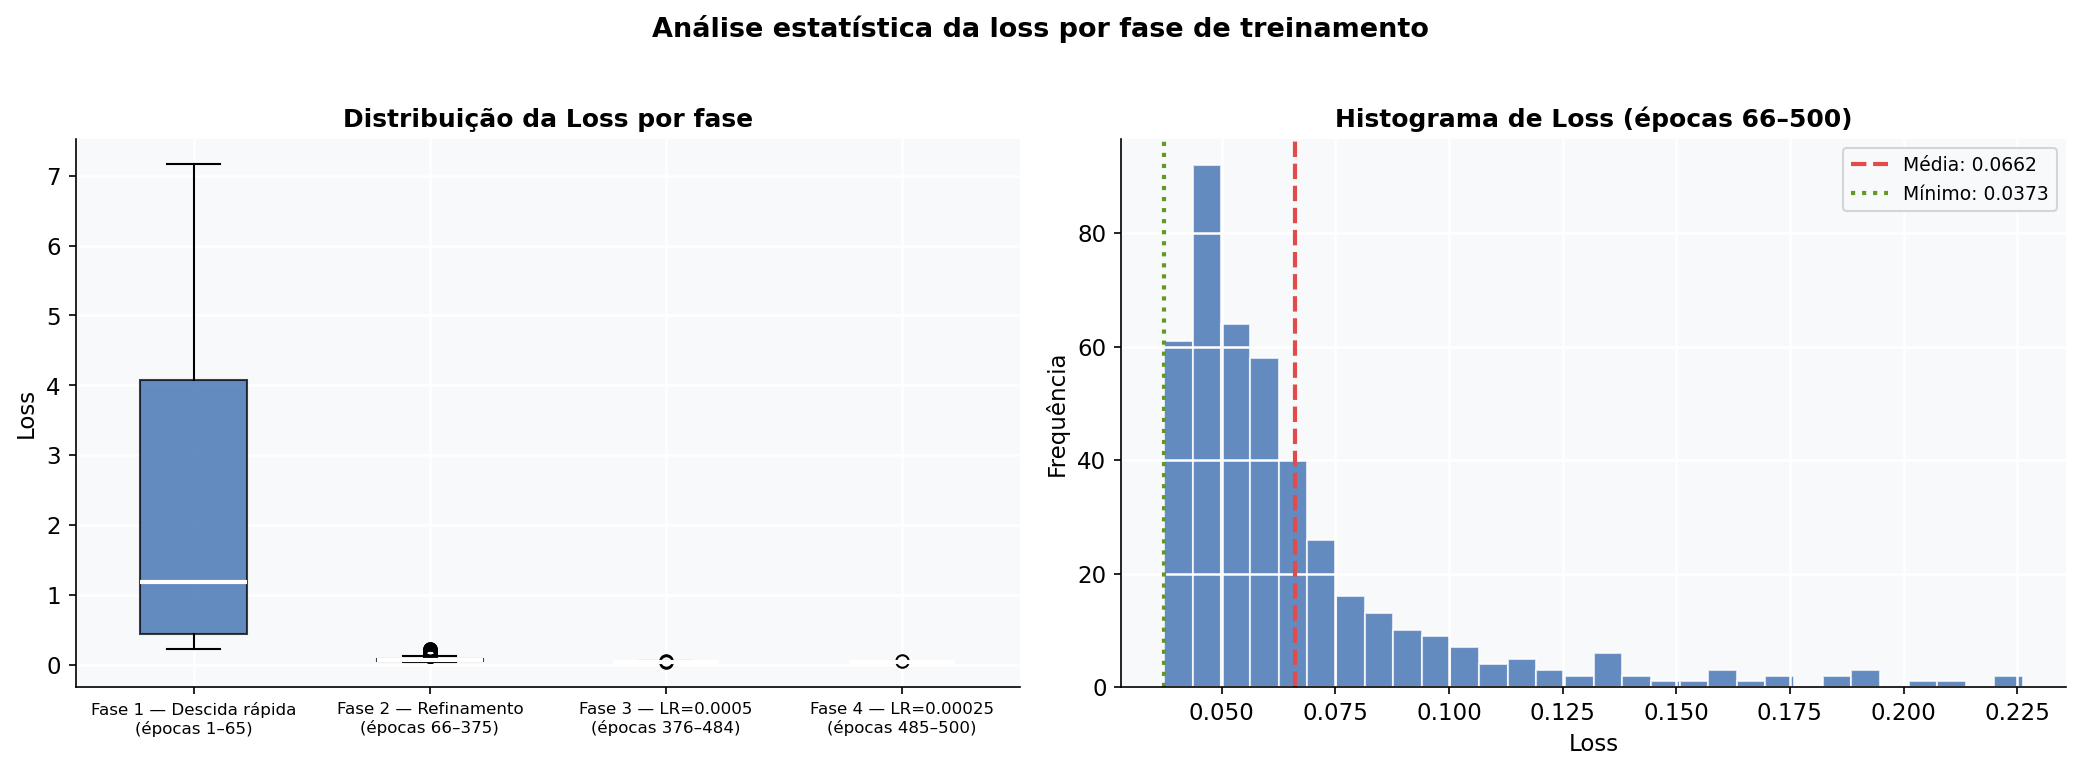
\includegraphics[width=16cm]{figuras/moco/distribuicao_loss}}
	}{
		\Fonte{elaborado pelo autor (2016).}
	}
\end{figure}

\begin{figure}[h!]
	\captionsetup{width=16cm}
	\Caption{\label{fig:loss_detalhada} Gráfico de tensão considerando a impedância humana}
	%\centering
	\UFCfig{}{
		\fbox{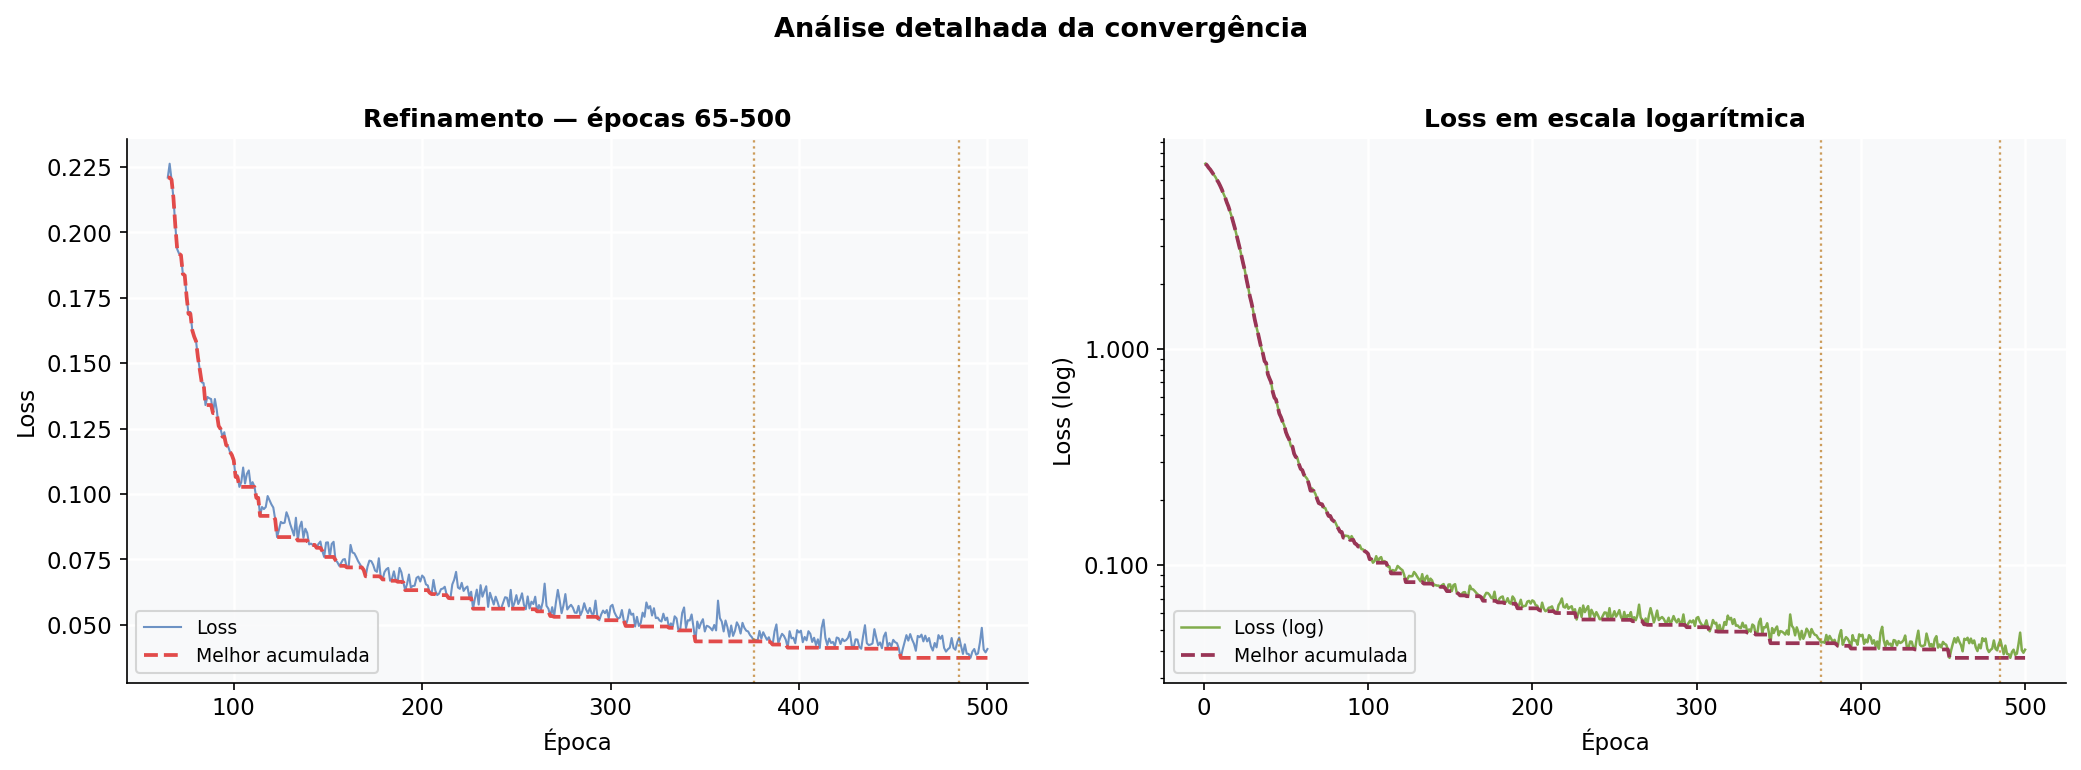
\includegraphics[width=16cm]{figuras/moco/loss_detalhada}}
	}{
		\Fonte{elaborado pelo autor (2016).}
	}
\end{figure}


\begin{figure}[h!]
	\captionsetup{width=16cm}
	\Caption{\label{fig:loss_geral} Gráfico de tensão considerando a impedância humana}
	%\centering
	\UFCfig{}{
		\fbox{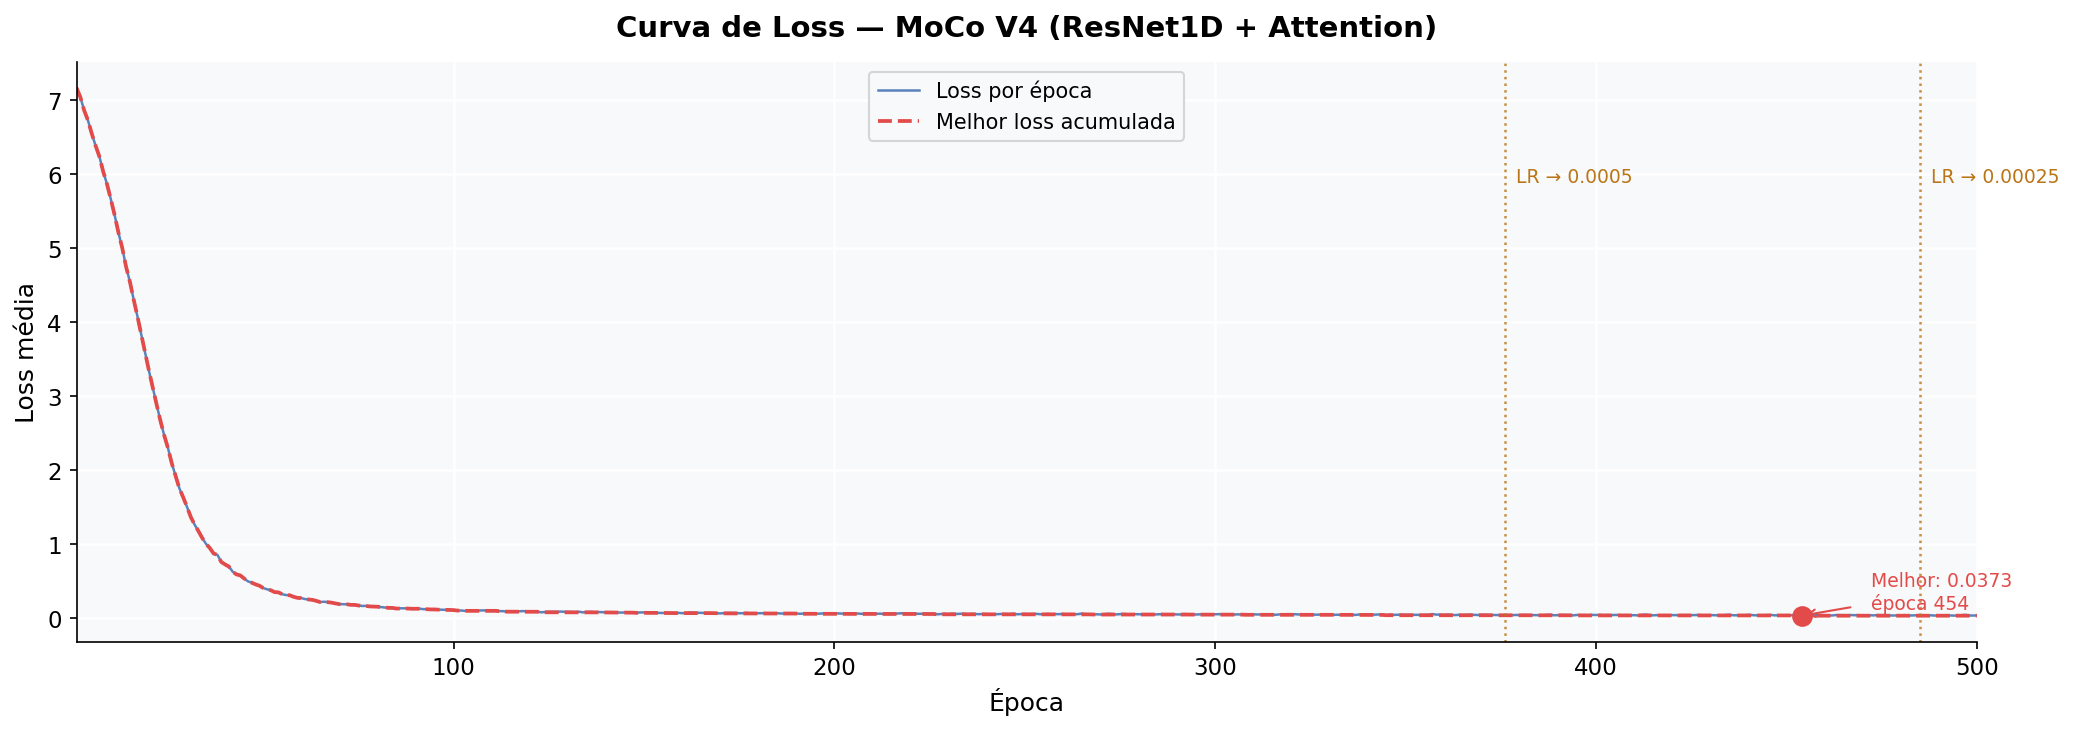
\includegraphics[width=16cm]{figuras/moco/loss_geral}}
	}{
		\Fonte{elaborado pelo autor (2016).}
	}
\end{figure}


\begin{figure}[h!]
	\captionsetup{width=16cm}
	\Caption{\label{fig:lr_loss} Gráfico de tensão considerando a impedância humana}
	%\centering
	\UFCfig{}{
		\fbox{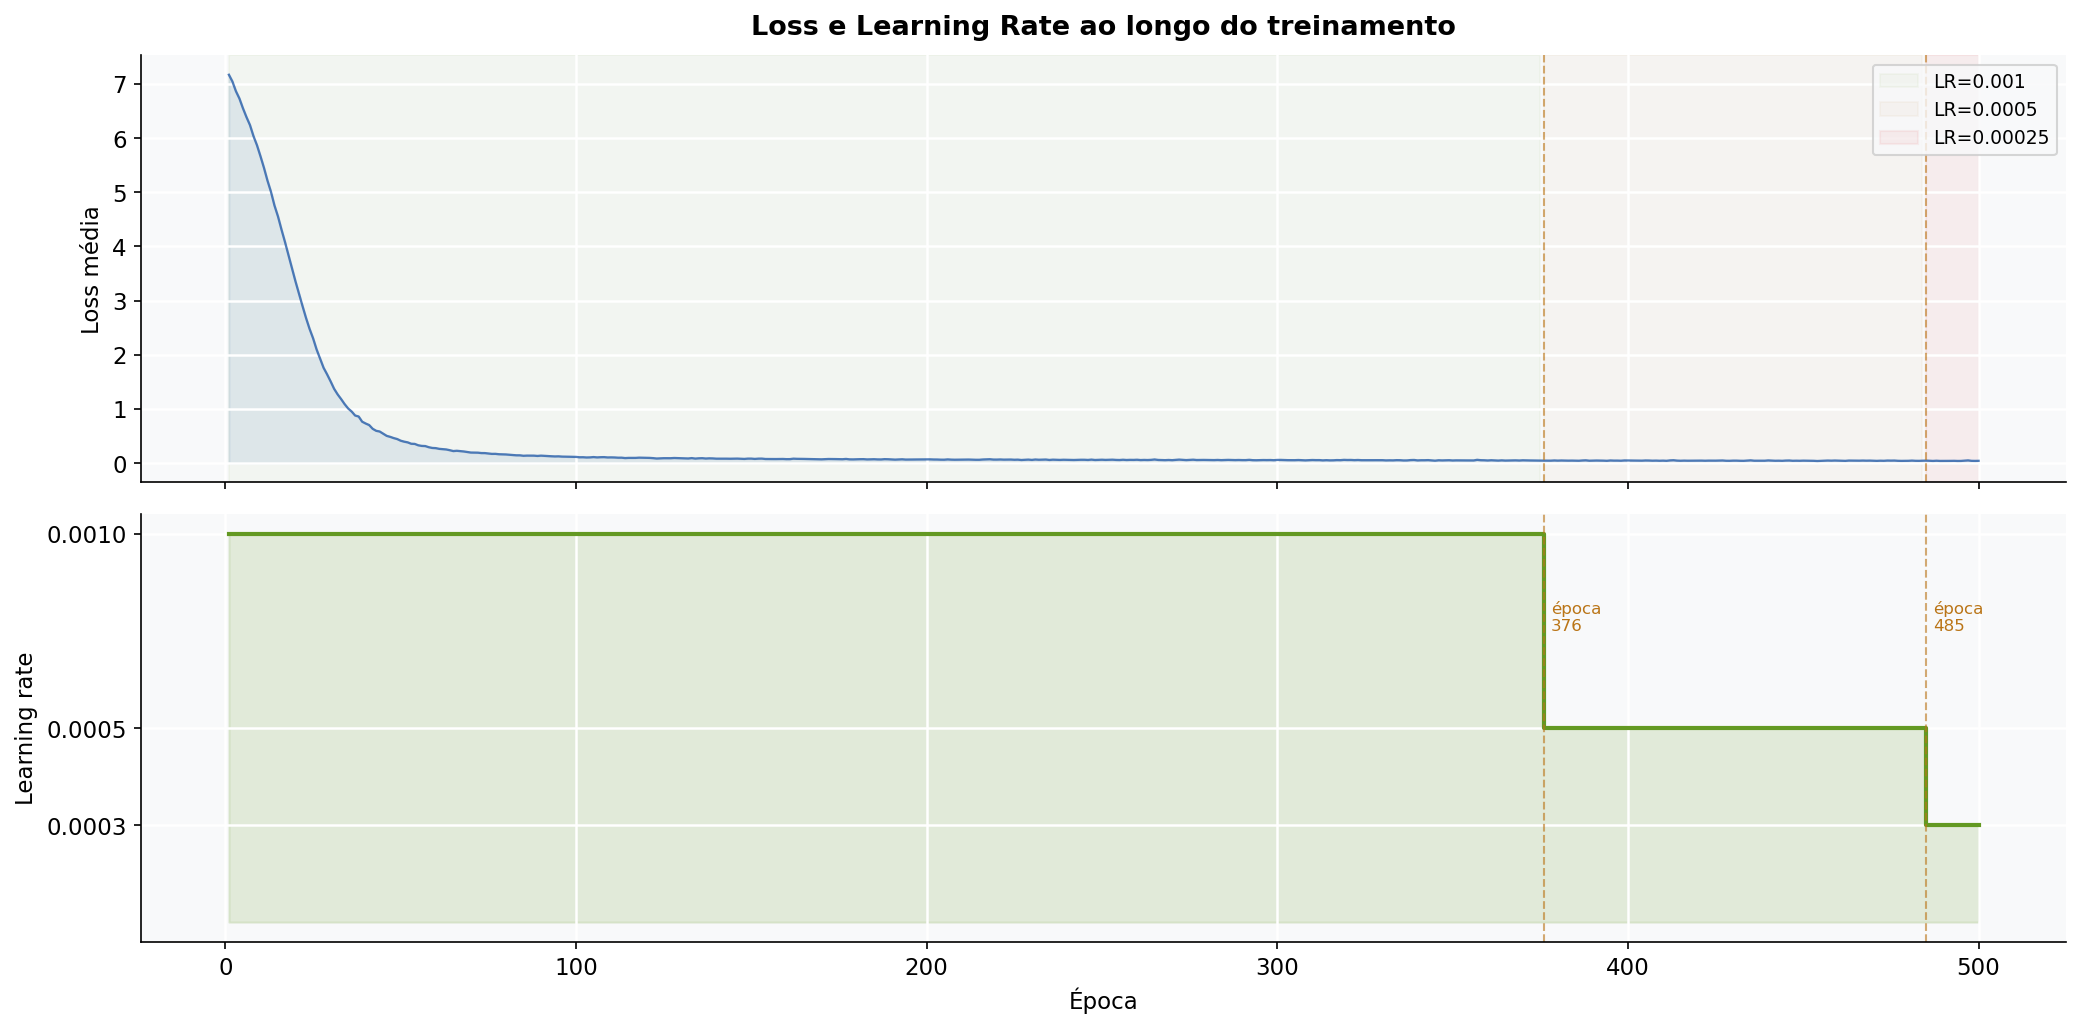
\includegraphics[width=16cm]{figuras/moco/lr_loss}}
	}{
		\Fonte{elaborado pelo autor (2016).}
	}
\end{figure}


\begin{figure}[h!]
	\captionsetup{width=16cm}
	\Caption{\label{fig:melhores_epocas} Gráfico de tensão considerando a impedância humana}
	%\centering
	\UFCfig{}{
		\fbox{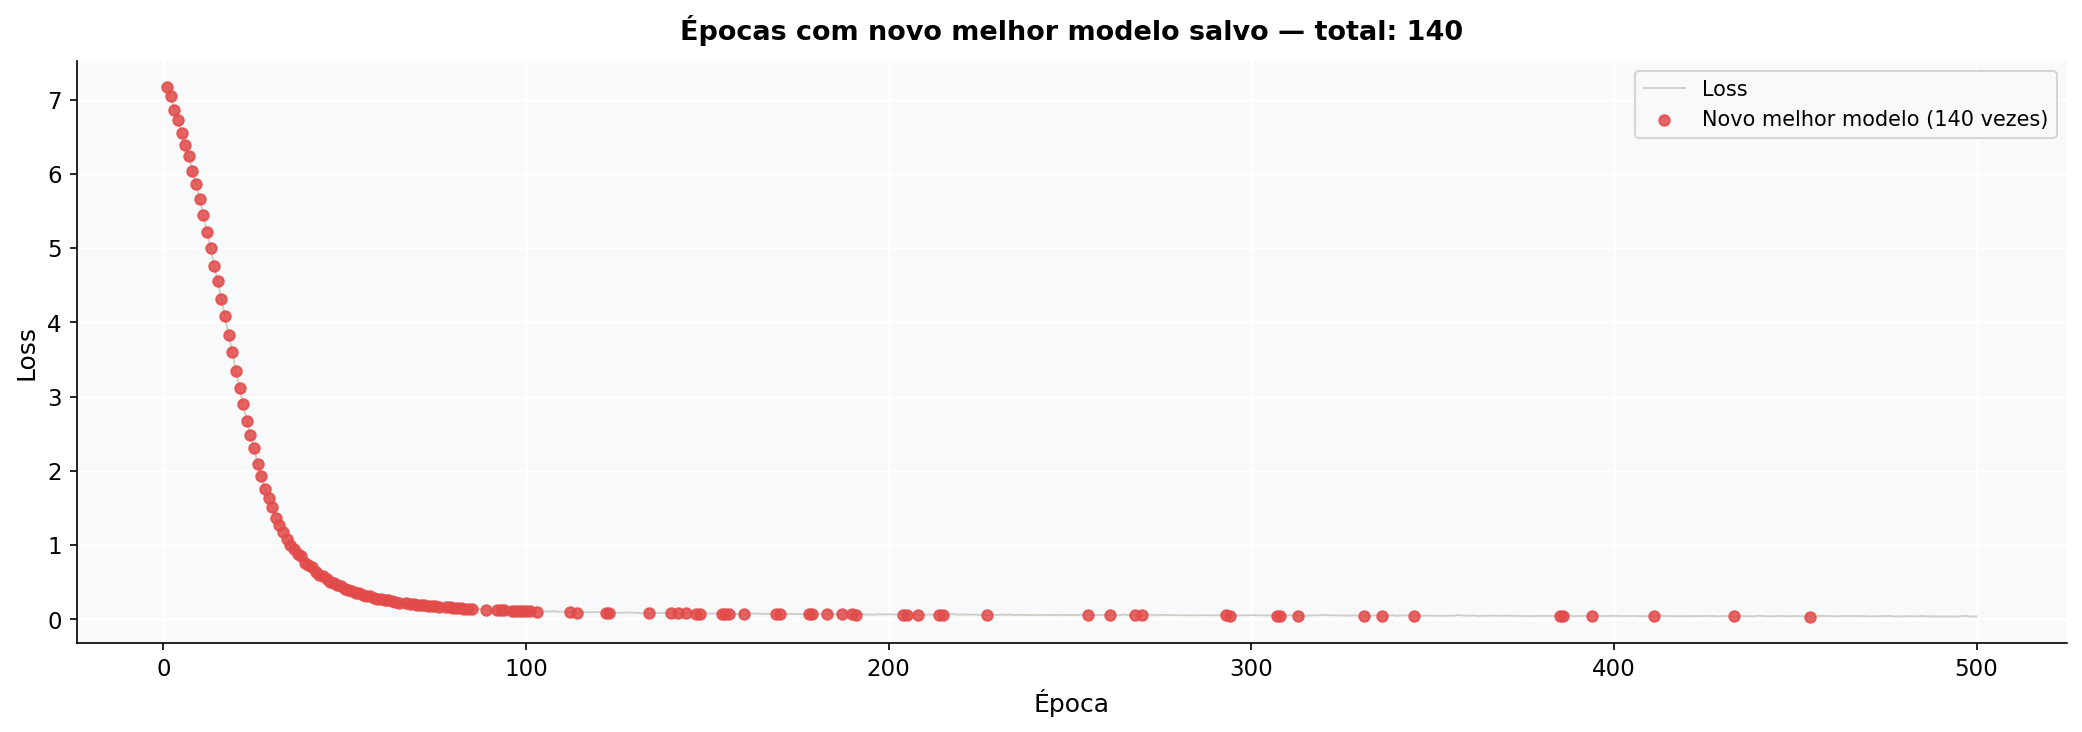
\includegraphics[width=16cm]{figuras/moco/melhores_epocas}}
	}{
		\Fonte{elaborado pelo autor (2016).}
	}
\end{figure}



\section{Resultados do Experimento A}
\label{sec:resultados-do-experimento-a}

Procure deixar as figuras dos resultados o maior possível preenchendo a largura do texto do documento que possui $16~cm$.

\begin{figure}[h!]
	\captionsetup{width=16cm}
	\Caption{\label{fig:tensaoimpedanciahumana} Gráfico de tensão considerando a impedância humana}
	%\centering
	\UFCfig{}{
		\fbox{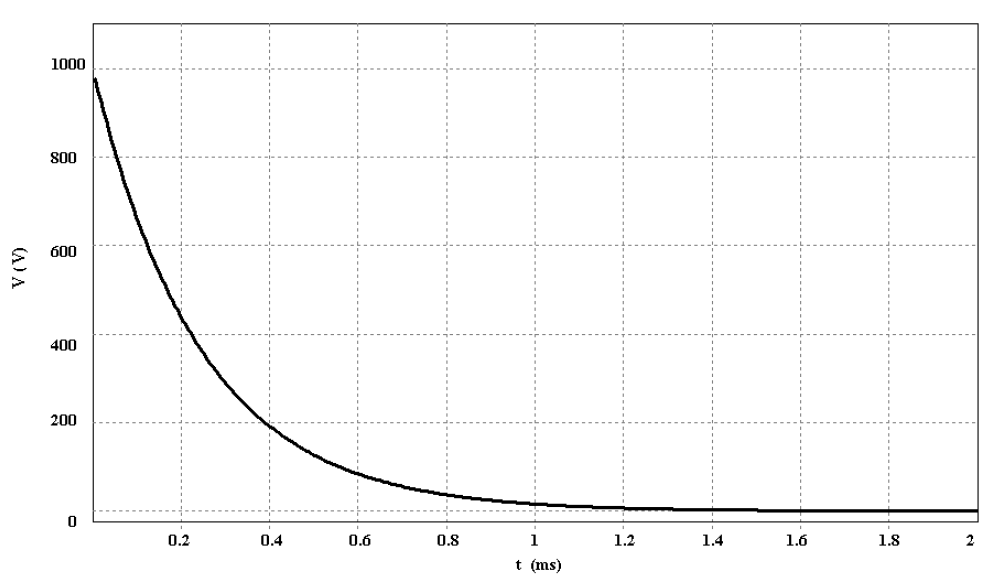
\includegraphics[width=16cm]{figuras/tensaoimpedanciahumana}}
	}{
		\Fonte{elaborado pelo autor (2016).}
	}
\end{figure}



Texto texto texto texto texto texto texto texto texto texto texto texto texto texto texto texto texto texto texto texto texto texto texto texto texto texto texto texto texto texto texto texto texto texto texto texto texto texto texto texto texto texto texto texto texto texto texto texto texto texto texto texto texto texto texto texto texto texto texto texto texto texto texto texto texto texto texto texto texto.

\begin{figure}[h!]
	\captionsetup{width=16cm}
	\Caption{\label{fig-grafico-1}Produção anual das dissertações de mestrado e teses de doutorado entre os anos de 1990 e 2008}
	\IBGEtab{}{
		\fbox{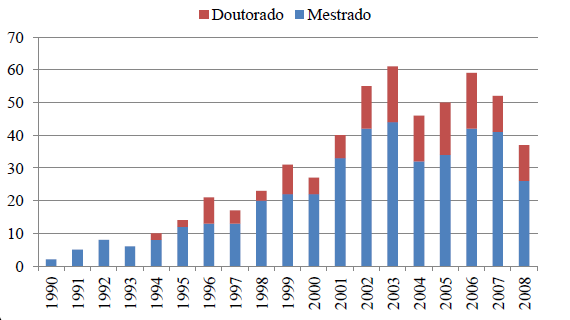
\includegraphics[width=16cm]{figuras/figura-3}}
	}{
		\Fonte{elaborado pelo autor (2016).}
	}
\end{figure}

Texto texto texto texto texto texto texto texto texto texto texto texto texto texto texto texto texto texto texto texto texto.

Texto texto texto texto texto texto texto texto texto texto texto texto texto texto texto texto texto texto texto texto texto texto texto texto texto texto texto texto texto texto texto texto texto texto texto texto texto texto texto texto texto texto texto texto texto texto texto texto texto texto texto texto texto texto texto texto texto texto texto texto texto texto texto texto texto texto texto texto texto.

\section{Resultados do Experimento B}
\label{sec:resultados-do-experimento-b}

Texto texto texto texto texto texto texto texto texto texto texto texto texto texto texto texto texto texto texto texto texto texto texto texto texto texto texto texto texto texto texto texto ..

\begin{table}[h!]
	%\centering
	\captionsetup{width=11.3cm}%ATENÇÃO: Ajuste a largura do título
	\Caption{\label{tab:notas} Notas dos participantes nas avaliações A, B e C}
	\IBGEtab{}{
		\begin{tabular}{crrr}
			\toprule
			Identificação dos participantes & Avaliação A & Avaliação B & Avaliação C \\
			\midrule \midrule
			Participante 1                  & 7           & 9           & 10          \\
			Participante 2                  & 8           & 2           & 1           \\
			Participante 3                  & 5           & 10          & 6           \\
			Participante 4                  & 3           & 1           & 4           \\
			Participante 5                  & 2           & 4           & 1           \\
			Participante 6                  & 0           & 7           & 2           \\
			\bottomrule
		\end{tabular}
	}{
		\Fonte{elaborado pelo autor (2016).}
	}
\end{table}



Texto texto Referenciando a \autoref{tab:notas}  texto texto texto texto texto texto texto texto texto texto texto texto texto texto texto texto texto texto texto texto texto texto texto texto texto texto texto texto texto texto.Texto texto texto texto texto texto texto texto texto texto texto texto texto texto texto texto texto texto texto texto texto.

Texto texto texto texto texto texto texto texto texto texto texto texto texto texto texto texto texto texto texto texto texto texto texto texto texto texto texto texto texto texto texto texto texto texto texto texto texto texto texto texto texto texto texto texto texto texto texto texto texto texto texto texto texto texto texto texto texto texto texto texto texto texto texto texto texto texto texto texto texto.Texto texto texto texto texto texto texto texto texto texto texto texto texto texto texto texto texto texto texto texto texto texto texto texto texto texto texto texto texto texto texto texto texto texto texto texto texto texto texto texto texto.

Texto texto texto texto texto texto texto texto texto texto texto texto texto texto texto texto texto texto texto texto texto texto texto texto texto texto texto texto texto texto texto texto texto texto texto texto texto texto texto texto texto texto texto texto texto texto texto texto.Texto texto texto texto texto texto texto texto texto texto texto texto texto texto texto texto texto texto texto texto texto.

Texto texto  Referenciando a \autoref{tab:notas}  texto texto texto texto texto texto texto texto texto texto texto texto texto texto texto texto texto texto texto texto texto texto texto texto texto texto texto texto texto texto texto texto texto texto texto texto texto texto texto texto texto texto texto texto texto texto texto texto texto texto texto texto texto texto texto texto texto texto texto texto texto texto texto texto texto texto texto.